\chapter{ДЕТАЛИ РЕАЛИЗАЦИИ}
\label{ch:ch2}

% \section{Практическая часть: введение}

Разработана библиотека ec.so, в которой реализованны возможности source-to-source компилятора языка Си.
К этой библиотеке написана небольшая утилита \verb|ecc|, реализующая для нее cli интерфейс.

\section{Интерфейс ecc}
\label{details:ecc-cli}
% Данная утилита(\verb|ecc|) является основным местом, куда пользователь идет при желании использовать компилятор.
Данная утилита(\verb|ecc|) является основным интерфейсом между пользователем и функционалом компилятора, реализованного в библиотеке \verb|ec.so|

\verb|ecc| использует библиотеку GNU Argp\cite{gnu-argp} для разбора и фильтрации аргументов, приходящих из командной строки. 
Argp автоматически генерирует сообщение[\ref{details:ecc-api:argp-usage-err}] об ошибке, при подаче неправильных аргументов.

\begin{lstlisting}[language=bash, caption={Пример сообщения об ошике, сгенерированного argp}, label={details:ecc-api:argp-usage-err}]
$ build/sandbox/ecc                                   
Usage: ecc [OPTION...] file...
Try `ecc --help' or `ecc --usage' for more information.
\end{lstlisting}

Так же argp добавляет ключ \verb|--help| и автоматически генерирует сообщение[\ref{details:ecc-api:argp-help}] со всеми основными ключами.
\begin{lstlisting}[language=bash, caption={Пример сообщения об использовании, сгенерированного argp}, label={details:ecc-api:argp-help}]
$ build/sandbox/ecc --help
Usage: ecc [OPTION...] file...
ecc - Extended C Compiler. Source-to-source compiler.

  -o, --output=FILE          Output to FILE instead of standard output
  -p, --proc-macro-file-path=<path>
                             Specify procedural macro file path
  -v, --verbose              Produce verbose output
  -?, --help                 Give this help list
      --usage                Give a short usage message
  -V, --version              Print program version

Mandatory or optional arguments to long options are also mandatory or optional
for any corresponding short options.
\end{lstlisting}

В случае успешного получения аргументов от \verb|arpg| \verb|ecc| далее просто вызывает соответствующие аргументам функции библиотеки \verb|ec|.


\section{Структура компиляции языка}
\label{passes}

Компиляция языка EC организована в виде последовательности проходов(passes), которые шаг за шагом преобразуют исходный текст программы в AST, 
трансформируют его, применяя макро-функции, переупорядочивая его, и транслируют в исходный код языка Си. 
Таким образом данный компилятор является source-to-source компилятором, т.к. преобразует исходный код одного языка к коду другого.

Проходы можно разделить на три группы:
\begin{itemize}
    \item Десериализирующие: к данной группе относятся проходы выводящие структуру из линейной последовательности элементов(символы, токены). 
    Сюда относятся проходы лексического[\ref{pass:lexing}] и грамматического разборов[\ref{pass:parsing}]
    \item Анализирующие и трансформирующие: к данной группе относятся проходы выполняющие манипуляции над AST деревом. 
    Сюда относятся проходы:
    \begin{itemize}
        \item Проходы регистрации и применения макросов[\ref{pass:macros}]
        \item Проход упорядочивания[\ref{pass:ordering}]
    \end{itemize}
    \item Сериализирующие: к данной группе относятся проходы уплощающие AST дерево в линейную последовательность элементов.
    Сюда относятся проходы:
    \begin{itemize}
        \item Проход трансляции в Си[\ref{pass:compile-c}]
        \item Проход трансляции в graphviz[\ref{pass:compile-dot}]
    \end{itemize}
\end{itemize}

В будущем планируется, что пользователь сможет добавлять свои проходы в процесс компиляции.

Далее в данной и последующих главах каждый из проходов будет рассмотрен в деталях.

Весь код приведенный в последующих главах оформлен в виде динамической библиотеки \verb|libec.so|.

\section{Компиляция синтаксического расширения}
Важное замечание, что \verb|@| директивы участвуют практически во всех приведенных выше[\ref{passes}] стадиях компиляции.

На этапе лексического разбора они есть только в виде составляющих их токенов 

На этапе грамматического разбора они - полноценный элемент AST, рассматривается их грамматика[\ref{parsing:at-directive:grammar}].

Каждый последующий этап интерпретирует свою часть директив. Потенциально пользователь библиотеки может дописывать свои директивы и этапы компиляции их использующие.
В данной работе реализованы этапы компиляции[\ref{pass:macros:compile}] и применения макросов[\ref{pass:macros:apply}], являющиеся примерами таких разработок.

До стадии трансляции в Си[\ref{pass:compile-c}] \textquote{доживают} только \verb|post_include| директивы, где транслируются в директивы препроцессора Си.





\clearpage
\section{Основные примитивы}
\label{primitives}

Библиотека реализованна на языке C23, используется некоторые улучшения, добавленные в новом стандарте.

Используются:
\begin{enumerate}
  \item ключевое слово \textbf{auto} для автоматического вывода типов
  \item взятие адреса у литерала, например \verb|&(int) {3}|
  \item gcc выражения-утверждения (statement expressions) вида \verb|({x = 3; x;})|
  \item gcc \verb|,##| оператор в макросах
\end{enumerate}

Для написания основной библиотеки используются дочерняя библиотека[\ref{extras:c-core}] с основными примитивами: 
строковыми, ввода-вывода, аллокации памяти и др.

Данная библиотека реализована в виде единичных самодостаточных заголовочных файлов, 
которые могут быть в зависимости от флага препроцессора либо заголовочными файлами либо файлами имплементации, 
по принципу stb библиотек\cite{stb_libs}.

Далее рассматриваю каждый примитив в отдельности:
\begin{itemize}
\item Макросы определения составных типов

Для определений структур и энумераций используются следующие макросы препроцессора Си[\ref{primitives:def-macros}]:
\begin{lstlisting}[language=c, caption={Макросы определения составных типов}, label={primitives:def-macros}]
#define struct_decl(name) \
typedef struct name name; \
struct name; \

#define enum_decl(name) \
typedef enum name name; \
enum name; \

#define struct_def(name, fields) \
typedef struct name name; \
struct name fields; \

#define enum_def(name, ...) \
typedef enum name name; \
enum name {__VA_ARGS__}; \
\end{lstlisting} 

Данные макросы позволяют не использовать соответствующее ключевое слово перед именем типа, 
например \verb|A| вместо \verb|struct A|.

\item Обработка ошибок


Ошибки кодируются как enum, например:

\begin{lstlisting}[language=c, caption={Ошибки Аллокатора}, label={primitives:error-enum-ex}]
enum_def(AllocatorError,
    ALLOCATOR_ERROR_OK,
    ALLOCATOR_ERROR_MEM_ALLOC,
    ALLOCATOR_ERROR_COUNT
)
#define ALLOCATOR_ERROR(ERR) ((AllocatorError)ALLOCATOR_ERROR_##ERR)
\end{lstlisting}

Значение OK кодируется как 0, остальные значения кодируются положительными числами.

Для обработки ошибок используются следующие макросы:
% \begin{minted}[linenos, frame=single]{c}
\begin{lstlisting}[language=c, caption={Макросы обработки ошибок}, label={primitives:error-macros}]
#define IS_OK(expr) ...
#define IS_ERR(expr) ...
#define TRY(expr) ...
#define ASSERT(expr) ...
#define ASSERTM(expr, msg) ...
#define ASSERT_OK(expr) ...
#define DBG_ASSERT(expr) ...
\end{lstlisting}

Где
\begin{itemize}
    \item \verb|IS_OK| - возвращает \verb|true|, если не было ошибки в данном выражении.

    \item \verb|IS_ERR| - возвращает \verb|true|, если была ошибка в данном выражении.

    \item \verb|TRY| - если в данном выражение была ошибка, то возвращает ошибку из текущей функции ключевым словом \verb|return|.

    \item \verb|ASSERT| - если выражение ложно, то критически завершает программу, используя вызов функции \verb|panic|.
    Данный примитив используется для проверки инвариантов во время работы программы и не убирается в \verb|release| режиме сборки.

    \item \verb|ASSERTM| - ведет себя также как \verb|ASSERT|, но позволяет дополнительно передать сообщение об ошибке.

    \item \verb|ASSERT_OK| - идентичен композиции \verb|ASSERT(IS_OK(expr))|.
    Является аналогом метода \verb|unwrap| в языке Rust.

    \item \verb|DBG_ASSERT| - аналог \verb|ASSERT|, убирающийся в \verb|release| режиме сборки.
\end{itemize}

\item Контекст

Используется глобальный контекст, уникальный для каждого потока:

\begin{lstlisting}[language=c, caption={Структура глобального контекста}, label={primitives:g_ctx-struct}]
__thread struct {
    Allocator global_alloc;

    StreamWriter stdout_sw;
    StreamWriter stderr_sw;
} g_ctx;
\end{lstlisting} 

Данный контекст содержит глобальный аллокатор[\ref{primitives:allocator}], и потоки вывода для \verb|stdout|, \verb|stderr|.

\item\label{primitives:allocator} Аллокатор

Используется интерфейс абстрактного аллокатора:

\begin{lstlisting}[language=c, caption={Интерфейс абстрактного аллокатора}, label={primitives:allocator-api}]
AllocatorError
allocator_alloc(Allocator* self, usize_t size, usize_t alignment, void **out_ptr);
AllocatorError
allocator_resize(Allocator* self, usize_t size, usize_t alignment, void **in_out_ptr);
allocator_free(Allocator* self, void **ptr);

AllocatorError
allocator_alloc_z(Allocator* self, usize_t size, usize_t alignment, void **out_ptr);
\end{lstlisting} 

Где данные функции работают аналогично функциям \verb|glibc| \verb|malloc|, \verb|resize|, \verb|free|, \verb|calloc| соответственно.
Однако они также поддерживаю произвольное выравнивание типа.

Примерами такого аллокатора служат глобальный glibc аллокатор и арена аллокатор[\ref{primitives:arena}].

\item\label{primitives:arena} Арена Памяти

Для оптимизации и удобства работы с памятью используется тип арены памяти \verb|Arena|, реализующая интерфейс абстрактного аллокатора.
Арена заранее выделяет большой кусок(chunk) памяти и при запросе на выделение памяти(функцией \verb|arena_alloc|) дает указатель внутри него. Если текущего куска недостаточно выделяется еще один и т.д.
Все куски хранятся как связанный список.

При запросе на освобождение(функцией \verb|arena_free|) памяти ничего не происходит. Арена очищает всю память разом при вызове метода \verb|arena_reset|.

Такой интерфейс позволяет удобно выделять память под задачи, имеющие определенное, конечное время жизни, как например этапы компиляции.

\item Строки

Привожу определения строк и строковых "срезов":

\begin{lstlisting}[language=c, caption={Строки и строковые срезы}, label={primitives:string-struct}]
struct_def(String, {
    uchar_t *ptr;
    usize_t byte_cap;
    usize_t byte_len; // in bytes
    Allocator allocator;
})

struct_def(str_t, {
    uchar_t *ptr;
    usize_t byte_len; // in bytes
})

typedef uint32_t rune_t;
\end{lstlisting}

Подразумевается, что \verb|String| владеет памятью, т.к. хранит абстрактный аллокатор, а \verb|str_t| нет.
Тип \verb|String| ведет себя в точности как динамический массив символов.

Подразумевается, что строки используют UTF-8 кодировку.

Тип \verb|rune_t| - unicode code point, число кодирующее символ в стандарте Юникод.

Строки - основной примитив использованный в данной работе. Они являются альтернативой Си строкам, которые не имеют поля длины и являются ноль-терминированными.
Для конвертации строковых литералов Си к типу \verb|str_t| используется макрос препроцессора Си: \verb|S(str)|.

При лексическом разборе[\ref{pass:lexing}] используется интерфейс итераторов считывания/записи юникод символов:
\begin{lstlisting}[language=c, caption={Функции итерации считывания/записи строк}, label={primitives:str-iter-api}]
UTF8_Error
str_next_rune(str_t self, rune_t *out_rune, str_t *out_self);
UTF8_Error
str_encode_next_rune(str_t self, rune_t rune, str_t *out_self);
\end{lstlisting}


\item Потоки вывода

Далее привожу интерфейс абстрактного потока вывода, использующийся для:

\begin{lstlisting}[language=c, caption={Интерфейс абстрактного потока вывода}, label={primitives:io-api}]
typedef IOError (StreamWriter_WriteFn)(void *, usize_t, uint8_t[]);
typedef IOError (StreamWriter_FlushFn)(void *);
\end{lstlisting}


Тип \verb|OutputFileStream| - поток вывода в файл, реализующий приведенный ранее интерфейс.
Строки тоже реализуют этот интерфейс(приведено с имплементацией).

\begin{lstlisting}[language=c, caption={Реализация интерфейса потока вывода другими типами}]
StreamWriter
output_file_stream_stream_writer(OutputFileStream *self);
StreamWriter
string_stream_writer(String *self);
\end{lstlisting}

\item\label{primitives:formatter} Форматирование строк

Для форматирования строк используется тип \verb|StringFormatter|, содержащий текущее состояние форматирования и настройки форматирования:
строку для индентации(например \verb|"    "|), выходной поток, куда форматтер выводит результат.

Основыные методы типа \verb|StringFormatter|:
\begin{lstlisting}[language=c, caption={Интерфейс объекта форматирования строк}, label={primitives:string-formatter-api}]
FmtError
string_formatter_write(StringFormatter *fmt, const str_t s);
FmtError
string_formatter_writeln(StringFormatter *fmt, const str_t s);
FmtError
string_formatter_write_fmt(StringFormatter *fmt, str_t fmt_str, ...);
\end{lstlisting}

Выше \verb|write_fmt| реализует функционал схожий с функцией \verb|glibc| \verb|printf|, 
добавлена поддержка строк типа \verb|str_t| и объектов реализующих интерфейс \verb|Formattable|[\ref{primitives:formattable-api}].

Интерфейс абстрактного форматируемого объекта \verb|Formattable|:
\begin{lstlisting}[language=c, caption={Интерфейс абстрактного форматируемого объекта}, label={primitives:formattable-api}]
FmtError 
formattable_fmt(Formattable *self, StringFormatter *fmt);
\end{lstlisting}


Используются следующие макросы для вывода в консоль:
\begin{lstlisting}[language=c, caption={Макросы для вывода в консоль}, label={primitives:print-macros}]
#define dbgp(___prefix, val, args...) ...
#define print_pref(___prefix, val) ...
#define println_pref(___prefix, val) ...

#define print_fmt(fmt_str, args...) ...                                 
#define println_fmt(fmt_str, args...) ...                               

#define eprint_fmt(fmt_str, args...) ...                                
#define eprintln_fmt(fmt_str, args...) ...                              
\end{lstlisting}

Где
\begin{itemize}
    \item \verb|dbgp| - макрос отладочного вывода. Вызов вида \verb|dbgp(foo, val, args...)| вызовет функцию отладочного форматирования \verb|foo_dbg_fmt|(ожидается, что она существует).
    \item \verb|print_pref| - макрос вывода в стандартный поток вывода по префиксу функции. Вызов вида \verb|print(foo, val)| вызовет функцию форматирования объекта \verb|foo_fmt|(ожидается, что она существует).
    \item \verb|println_pref| - аналогичен \verb|print_pref|, но пишет символ переноса строки в конце.

    \item \verb|print_fmt| - работает аналогично функции \verb|glibc| \verb|printf|, но вместо строк Си использует строки типа \verb|str_t|, также поддерживает абстрактные форматируемые объекты.
    \item \verb|println_fmt| - аналогичен \verb|print_fmt|, но пишет символ переноса строки в конце.
    
    \item \verb|eprint_fmt| - аналогичен \verb|print_fmt|, но пишет в стандартный поток ошибок.
    \item \verb|eprintln_fmt| - аналогичен \verb|println_fmt|, но пишет в стандартный поток ошибок.
\end{itemize}

\item Структуры данных

Далее в работе активно используются следующие структуры данных:
\begin{itemize}
    \item \verb|slice_t| - статический массив, выполнен как указатель и кол-во элементов.
    \item \verb|darr_t| - динамический массив, владеет паматью и хранит абстрактный аллокатор.
    \item\label{primitives:hashmap} \verb|hashmap_t| - хеш-таблица.
    \item \verb|hashset_t| - хеш-множество.
\end{itemize}


Для каждого из них существует аналогичный макрос с окончанием \verb|_T|, позволяющий указывать имена типов, находящихся в контейнере.
Например \verb|darr_T(int)| - динамический массив целых чисел, \verb|hashmap_T(str_t, Foo)| - хеш-таблица с ключами типа \verb|str_t| и со значениями типа \verb|Foo|.

%

% \newpage
% \subsection{Интерфейс работы с узлом трансляции}

% В библиотеке есть высокоуровневая абстракция единицы трансляции, на которой реализованны функции преобразований(прохов/passes).


% \beginminteddef{c}
% struct_def(C_TranslationUnitData, {
%     str_t main_file;
%     hashmap_T(str_t, TU_FileData) file_data_table;
%     // lexing
%     darr_T(C_Token) tokens;
%     // parsing
%     C_Ast_TranslationUnit *tr_unit;

%     // analysis
%     C_SymbolTable symbol_table;
%     // hashmap_T(str_t, void) topsort_start_symbols;
% #ifdef EXTENDED_C
%     C_SymbolTable proc_macro_table;
%     void *proc_macro_lib; // handle from dlopen call
% #endif // EXTENDED_C

%     // mem
%     Arena string_arena;
%     Arena token_arena;
%     Arena ast_arena;
% })

% void
% c_translation_unit_init(C_TranslationUnitData *self, str_t main_file_path);
% void
% c_translation_unit_deinit(C_TranslationUnitData *self);
% bool
% c_translation_unit_lex(C_TranslationUnitData *self);
% bool
% c_translation_unit_parse(C_TranslationUnitData *self);
% void
% ec_translation_unit_ast_unparse(C_TranslationUnitData *self, StreamWriter *dst_sw);
% void
% ec_translation_unit_ast_compile_graphvis(C_TranslationUnitData *self, StreamWriter *dst_sw);
% \end{minted}

% Примеры использования данного иМнтерфейса: % TODO
\end{itemize}

\chapter{СИНТАКСИЧЕСКИЙ АНАЛИЗ}

Синтаксический анализ текста программы EC происходит в два этапа: 
\begin{enumerate}
    \item лексический анализ
    \item грамматический разбора
\end{enumerate}

Этапы рассмотрены соответственно в параграфах \ref{pass:lexing} и \ref{pass:parsing}.

% \clearpage
\section{Лексический анализ}
\label{pass:lexing}

Лексический разбор выполняет преобразование из последовательности символов в последовательность токенов(лексем), в соответствии с лексической грамматикой.
Для Си данная грамматика приведена в стандарте\cite{c99_std} (Annex A, 1. Lexical Grammar), и является LL(1) грамматикой.

Выполненный токенизатор(лексер, сканнер) языка Си является LL(2) парсером, т.к. использует до двух look-ahead токенов.

\section{Структура токена Си}

Токен Си - лексема, единица лексического разбора.

\begin{lstlisting}[language=c, caption={Структура токена Си}, label={lexing:c-token-struct}]
struct_def(C_Token, {
    C_TokenKind kind;
    C_LexerSpan span;
    C_TokenFlags flags;
    union {
        C_TokenIdent t_ident;
        C_TokenKeyword t_keyword;
        C_TokenPunct t_punct;
        C_TokenComment t_comment;
        C_TokenStringLiteral t_str_lit;
        C_TokenCharLiteral t_char_lit;
        C_TokenNumLiteral t_num_lit;
        C_Token_PP_Directive t_pp_directive;
        C_TokenHeaderName t_header_name;
        C_TokenInclude t_include;
        C_TokenExpand t_expand;
    };
})
\end{lstlisting}

Тип \verb|C_Token| является объединением конкретных типов токенов, таких как
\begin{itemize}
  \item \verb|C_TokenIdent| - идетификатор, например:
  \verb|x|, \verb|y|, \verb|z|

  \item \verb|C_TokenKeyword| - ключевое слово, например:
  \verb|int|, \verb|return|, \verb|auto| \\
  список ключевых слов приведен в приложении[\ref{extras:c_defs}]

  \item \verb|C_TokenPunct| - знак препинания(пунктуатор), например:
  \verb|;|, \verb|{|, \verb|++|

  \item \verb|C_TokenComment| - комментарий, например:
  \verb|// comment|, \verb|/* muliline comment */|

  \item \verb|C_TokenStringLiteral| - строковой литерал, например: \verb|"text"|
  \item \verb|C_TokenCharLiteral| - символьный литерал, например: \verb|'\u20ac'|
  \item \verb|C_TokenNumLiteral| - числовой литерал, например: \verb|'0x1234abcdeful'|
  \item \verb|C_TokenNumLiteral| - числовой литерал, например: \verb|'0x1234abcdeful'|

  Последующие токены относятся к препроцессору и будут рассмотренны далее[\ref{pass:pp}]
  \item \verb|C_Token_PP_Directive|
  \item \verb|C_TokenHeaderName|
  \item \verb|C_TokenInclude|
  \item \verb|C_TokenExpand|
\end{itemize}

В \verb|int x = 3;|: 
\begin{itemize}
    \item \verb|int| - ключевое слово 
    \item \verb|x| - идетификатор 
    \item \verb|=| и \verb|;| - знаки препинания 
    \item \verb|3| - числовой литерал
\end{itemize}

Вид конкретного токена определяется полем \verb|kind| структуры \verb|C_Token|.
\begin{lstlisting}[language=c, caption={Виды токенов Си}, label={lexing:kind-enum}]
enum_def(C_TokenKind, 
    C_TOKEN_KIND_INVALID,
    C_TOKEN_KIND_IDENT,
    C_TOKEN_KIND_KEYWORD,
    C_TOKEN_KIND_STRING,
    C_TOKEN_KIND_CHAR,
    C_TOKEN_KIND_NUMBER,
    C_TOKEN_KIND_PUNCT,
    C_TOKEN_KIND_COMMENT,
    C_TOKEN_KIND_PP_DIRECTIVE,
    C_TOKEN_KIND_INCLUDE,
    C_TOKEN_KIND_EXPAND,
    C_TOKEN_KIND_NEW_LINE,
    C_TOKEN_KIND_EOF
)
\end{lstlisting}


% Также \verb|C_Token| содержит мета информацию о расположении в исходном файле.
Поле \verb|span| - содержит информацию о расположении токена в исходном файле: начальные и конечные сдвиг в тексте, номер линии, номер столбца.

Поле \verb|flags| - содержит флаги, такие как:
\begin{itemize}
    \item \verb|WAS_SPACE| - был ли пробел(любой символ, пустого пространства) после предыдущего токена.
    \item \verb|WAS_NEW_LINE| - была ли новая строка после предыдущего токена.
\end{itemize}

Полный код токена приведен в приложении[\ref{extras:c_token}]

% \section{Структура состояния разбора}

Основная структура лексического анализа, содержащая состояние разбора:
\begin{lstlisting}[language=c]
struct_def(LexerState, { ... })
\end{lstlisting}

Она содержит следующие важные поля:
\begin{itemize}
  \item \verb|text| - указатель на разбираемый текст
  \item \verb|rest| - оставшаяся подстрока в тексте

  \item \verb|line|, \verb|col|, \verb|flags| - текущие строка, столбец, флаги соответственно
  \item далее идут настройки препроцессора
  
  \item \verb|token_arena|, \verb|string_arena| - арены памяти для токенов и строк соответственно
  \item \verb|string_batch| - строковый буффер для построения строк

  \item далее идут изменяемые обработчики ошибок
\end{itemize}

\section{Функции лексического анализа}
\label{lexing:fns}

Главная функция токенизатора, где определяется вид следующей лексемы, выполнена в виде итератора.

\begin{lstlisting}[language=c]
LexingError
lexer_next_token(LexerState *state, C_Token *out_token);
\end{lstlisting}

Ее использует функция \verb|tokenize|, собирающая все токены в массив.
\begin{lstlisting}[language=c]
LexingError
tokenize(LexerState *state, darr_T(C_Token) *out_tokens);
\end{lstlisting}

Разбор выполняется с помошью двух основных функций:
\begin{lstlisting}[language=c]
INLINE
rune_t
lexer_peek_rune(LexerState *state);
rune_t
lexer_advance_rune(LexerState *state);
\end{lstlisting}

\verb|lexer_peek_rune| - посмотреть текущий символ \\
\verb|lexer_advance_rune| - продвинуться вперед на один символ \\
иногда используется \verb|lexer_peek_rune2| - посмотреть следующий за текущим символ

Привожу пример функции лексического разбора:
\begin{lstlisting}[language=c, caption={Пример функции лексического разбора}, label={lexing:fn-ex}]
LexingError
lex_ascii_char_set(LexerState *state, ASCII_CharSet set, uchar_t *out_char) {
    rune_t r = lexer_peek_rune(state);
    if (r > 256) {
        return LEXING_ERROR(NONE);
    }
    uchar_t c = (uchar_t)r;
    if (!ascii_char_set_is_in(c, set)) {
        return LEXING_ERROR(NONE);
    }

    lexer_advance_rune(state);
    *out_char = c;
    return LEXING_ERROR(OK);
}
\end{lstlisting}

Данная функция принимает на вход состояние(\verb|state|), и множество символов(\verb|set|), представленное в виде битового поля,
проверяет принадлежит ли текущий символ множеству \verb|set|, и в случае принадлежности возвращает символ через указатель \verb|out_ptr|,
и переводит состояние(\verb|state|) на следующий символ.

Если функция отработала успешно (текущий символ принадлежит множеству \verb|set|), то возвращается \verb|OK|, в противном случае \verb|NONE|.
В зависимости от возвращенного значения вызывающая функция (caller) решает, что делать дальше.

Похожим образом работают все функции лексического разбора.
Некоторые из них приведены в приложении[\ref{extras:lexer_fns}]

\clearpage
\section{Пример использования токенизатора}

Для демонстрации полученных токенов, написана функция отладочного вывода \verb|dbg_print_tokens|[\ref{extras:token_dbg_print}]

Напишем маленький пример, использующий функцию\newline \verb|dbg_print_tokens|
\begin{lstlisting}[language=c, caption={Пример использования лексера}, label={lexing:lexer-usage-ex}]
    str_t text = S(
        "int x = y + 3;"
        );
    LexerState state;
    lexer_init_default(&state, text, S("<file>"));
    darr_t tokens;
    ASSERT_OK(tokenize(&state, &tokens));
    dbg_print_tokens(tokens, text, state.file_data_table);
    darr_free(&tokens);
    lexer_deinit(&state);
}
\end{lstlisting}

Код в переменной \verb|text|:
\begin{lstlisting}[language=c, caption={Входные данные примера}, label={lexing:usage-ex-in}]
int x = y + 3;
\end{lstlisting}

Вывод:

\begin{lstlisting}[language=bash, caption={Входные данные примера}, label={lexing:usage-ex-out}]
Token:
    kind: C_TOKEN_KIND_KEYWORD,
    flags: 0,
    span: 0(1:1) - 3(1:4) [<file>],
    text: int
Token:
    kind: C_TOKEN_KIND_IDENT,
    flags: 1,
    span: 4(1:5) - 5(1:6) [<file>],
    text: x
Token:
    kind: C_TOKEN_KIND_PUNCT,
    flags: 1,
    span: 6(1:7) - 7(1:8) [<file>],
    text: =
Token:
    kind: C_TOKEN_KIND_IDENT,
    flags: 1,
    span: 8(1:9) - 9(1:10) [<file>],
    text: y
Token:
    kind: C_TOKEN_KIND_PUNCT,
    flags: 1,
    span: 10(1:11) - 11(1:12) [<file>],
    text: +
Token:
    kind: C_TOKEN_KIND_NUMBER,
    flags: 1,
    span: 12(1:13) - 13(1:14) [<file>],
    text: 3
Token:
    kind: C_TOKEN_KIND_PUNCT,
    flags: 0,
    span: 13(1:14) - 14(1:15) [<file>],
    text: ;
Token:
    kind: C_TOKEN_KIND_EOF,
    flags: 0,
    span: 14(1:15) - 14(1:15) [<file>],
    text: unimplemented
\end{lstlisting}

\clearpage
\section{Препроцессор}
\label{pass:pp}

Препроцессор интегрирован с лексером(функция \verb|tokenize|) и использует лексер как итератор.
Препроцессор опциональный, включается флагом \verb|do_preprocessing| структуры \verb|LexerState|.
Реализицию препроцессора можно посмотреть в приложении[\ref{extras:pp}].

При работе препроцессора, директивы \verb|#include| заменяются токеном \verb|C_TokenInclude|, \\
дерективы \verb|#define| регистрируют токены макроса в хеш-таблице \verb|LexerState::pp_defs|, \\
дерективы \verb|#ifdef|, \verb|#ifndef|, \verb|#else|, \verb|#endif| условно влючают или исключают блоки кода, 
с помощью \verb|LexerState::pp_if_depth|(глубина \verb|#if| стека) и \verb|LexerState::pp_defs|, \\
идентификаторы проверяются на наличие в таблице \verb|LexerState::pp_defs|, и при наличи заменяются токеном \verb|C_TokenExpand|,
при этом замена производится рекурсивно.

Приведем пример работы препроцессора:

В построенный выше пример[\ref{lexing:lexer-usage-ex}] подставляем следующий код языка Си:
\begin{lstlisting}[language=c, caption={Входные данные примера}, label={lexing:pp:ex-in}]
#define A a
#define B A b
#define C B c
#ifdef C
#define D d
#endif

C D
\end{lstlisting}

Получаем следующую последовательность токенов:
\begin{lstlisting}[language=bash, caption={Выходные данные примера}, label={lexing:pp:ex-out}]
Token:
    kind: C_TOKEN_KIND_IDENT,
    flags: 1,
    span: 10(1:11) - 11(1:12) [<file>],
    text: a
Token:
    kind: C_TOKEN_KIND_IDENT,
    flags: 1,
    span: 24(2:13) - 25(2:14) [<file>],
    text: b
Token:
    kind: C_TOKEN_KIND_IDENT,
    flags: 1,
    span: 38(3:13) - 39(3:14) [<file>],
    text: c

Token:
    kind: C_TOKEN_KIND_IDENT,
    flags: 1,
    span: 59(5:11) - 60(5:12) [<file>],
    text: d

Token:
    kind: C_TOKEN_KIND_EOF,
    flags: 0,
    span: 71(7:4) - 71(7:4) [<file>],
    text: unimplemented
\end{lstlisting}

Заметим, что в выходных данных[\ref{lexing:pp:ex-out}] мы не видим токенов типа \verb|C_TokenExpand|, 
т.к. функция \verb|dbg_print_tokens|[\ref{lexing:lexer-usage-ex}] итерирует по вложенной структуре, выводя \textquote{плоский} результат.

\section{Постобработка}

На данном этапе, после препроцессора, у нас получилась потенциально древовидная(вложенная) структура.
Чтобы итерировать по вложенной структуре нужен стек, что добавляет дополнительные затраты(overhead), 
плюс возвращение парсера к контрольной точке становится потенциально тяжеловесной операцией(приходится копировать весь стек).
Это происходит в связи с тем, что нельзя предсказать как токены Си будут распределены по макросам препроцессор Си.


% Все было бы не так плохо если бы макросы не были бы столь неогранниченными, например:

% Может быть, что элемент грамматики Си разбит на несколько макросов вот так:
% \beginminteddef{c}
% #define BE if (1) {
% #define EN }

% BE
% // code
% EN
% \end{minted}

% и при откате может потребоваться вернуть часть стека поверх, что нетривиально.
% если добавить ограничение, что макрос может содержать только сбалансированные скобки ('{', '}'), тогда

Поэтому было принято решение уплощить вложенную структуру.

Функции выполняющие это:
\begin{lstlisting}[language=c, caption={Заголовки функций уплощения}, label={lexing:flat-fns}]
usize_t
_c_token_list_flatten_at(darr_T(C_Token) tokens, C_Token *dst);
AllocatorError
c_token_list_flatten_in(darr_T(C_Token) tokens, 
                        usize_t token_count_upper_bound, 
                        Allocator *alloc, darr_T(C_Token) *out_tokens); 
\end{lstlisting}

% диаграмма

Теперь все вышесказанное можно организовать в виде прохода:

\begin{lstlisting}[language=c, caption={Функция этапа лексического разбора}, label={lexing:pass-fn}]
bool
c_translation_unit_lex(C_TranslationUnitData *self) {
    ASSERT_OK(arena_init(&self->string_arena, 4096, ctx_global_alloc));
    ASSERT_OK(hashmap_new_cap_in_T(str_t, TU_FileData, 64, &g_ctx.global_alloc, &self->file_data_table));

    TU_FileData *fdata = nullptr;
    auto alloc = arena_allocator(&self->string_arena);
    ASSERT_OK(file_data_table_get_or_load_file(&self->file_data_table, self->main_file, nullptr, 
        &alloc, &fdata));

    ASSERT_OK(arena_init(&self->token_arena, str_len(fdata->text), ctx_global_alloc));

    LexerState lstate;
    _translation_unit_lexer_init(self, &lstate, fdata->text);

    if (IS_ERR(tokenize(&lstate, &self->tokens))) {
        return false;
    }

    darr_t flat;
    
    ASSERT_OK(c_token_list_flatten_in(self->tokens, 
        arena_total_size(&self->token_arena), &g_ctx.global_alloc, &flat));
    
    darr_free(&self->tokens);
    self->tokens = flat;

    _translation_unit_lexer_deinit(&lstate);
    return true;
}
\end{lstlisting}

% глава или параграф
Итак в данной главе были рассмотрены:
\begin{itemize}
  \item Структура токена Си
  \item Структура лексера Си
  \item Некоторые методы лексического разбора
  \item Препроцессор языка Си
  \item Постобработка - уплощение структуры токенов
\end{itemize}

% \section{Грамматический разбор}
% \label{pass:parsing}

% \section{Парсер Пратта}
% \label{pass:parsing:pratt}
% Парсер Пратта использует комбинацию циклов и рекурсивных вызовов функций.
% Есть хорошая статья, в которой приводится реализация данного парсера на языке Rust\cite{matklad_pratt_parsers}.

% Парсер Пратта для инфиксных операторов упрощенно работает по следующему принципу: 

% % \begin{lstlisting}[language=python, caption={Псевдокод алгоритма парсера Пратта}]
% % def parse_expr(state, max_precedence, flags) -> expr, err:
% %     left: Expr
    
% % \end{lstlisting}

% \begin{enumerate}
%     \item Начало определения рекурсивной функции \verb|parse_expr|, 
%     принимающей параметры состояния разбора \verb|state| и максимального значения порядка следования \verb|max_precedence|

%     \begin{itemize}
%         \item Пусть \verb|left: Expr| - переменная типа \verb|Expr|

%         \item В \verb|left| записывается первый аргумент или выходим с ошибкой, если его нет или он является именем типа

%         \item\label{pratt:alg:loop} Пока есть следующий за аргументом бинарный оператор, удовлетворяющий ограничениям порядка следования и ассоциативности:

%         \begin{itemize}
%             \item Разбираем оператор записываем в переменную \verb|op: Expr|

%             \item\label{pratt:alg:rec-call} Разбираем правый операнд выражения рекурсивным вызовом функции \verb|parse_expr|, 
%             со значением \verb|max_precedence| равным порядку следования оператора в переменной \verb|op|

%             \item Записываем в \verb|left| значение переменной \verb|op|
%         \end{itemize}
%     \end{itemize}

%     \item Конец определения функции \verb|parse_expr|
% \end{enumerate}


% Рекурсивные вызовы[\ref{pratt:alg:rec-call}] в алгоритме сами по себе разбирают цепочки операторов с убывающем номером порядка следования
% (или одинаковым при условии ассоциативности справа на лево). 
% Синтаксические деревья полученные после разбора таких операторов, являются наклоненными направо, как показано на диаграмме[\ref{pratt:right-lean-diag}].

% Тогда как цикл[\ref{pratt:alg:loop}] в алгоритме сам по себе разбирает цепочки операторов с оставшимися после рекурсивного вызова номерами порядка следования, 
% т.е. возрастающими или одинаковыми при условии ассоциативности слева на право. 
% Синтаксические деревья полученные после разбора таких операторов, являются наклоненными налево, как показано на диаграмме[\ref{pratt:left-lean-diag}].


% \begin{figure}[h!]
%     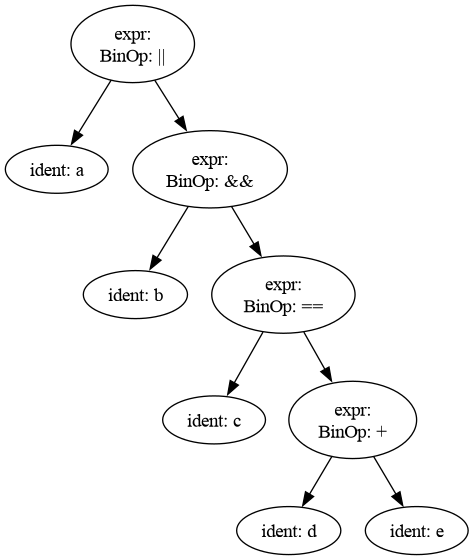
\includegraphics[width=\textwidth,height=\textheight,keepaspectratio]{right-lean-diag.png}
%     \centering
%     \caption{AST цепочки операторов с убывающим номером порядка следования}
%     \label{pratt:right-lean-diag}
% \end{figure}

% \begin{figure}[h!]
%     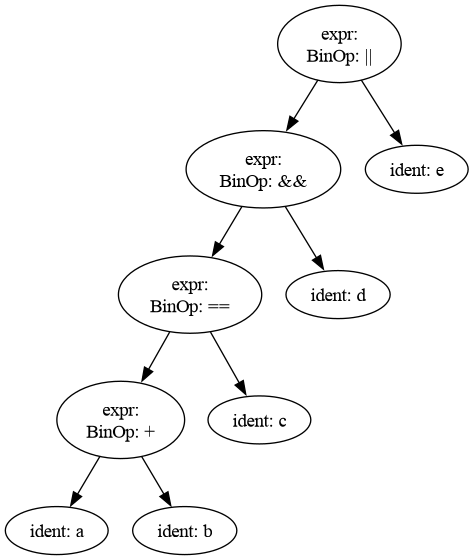
\includegraphics[width=\textwidth,height=\textheight,keepaspectratio]{left-lean-diag.png}
%     \centering
%     \caption{AST цепочки операторов с возрастающим номером порядка следования}
%     \label{pratt:left-lean-diag}
% \end{figure}


% \FloatBarrier




\clearpage
\section{Грамматический разбор}
\label{pass:parsing}

Далее будет рассмотрен грамматический разбор или парсинг потока токенов, получаемый после прохода лексера.
Грамматический разбор - процесс превращения потока(последовательности) лексических единиц в синтаксическое дерево, рассматриваемое далее[\ref{parsing:ast}].
Разбор производится методом рекурсивного спуска, который рассматривается далее[\ref{parsing:rec-desc}]. Для разбора выражений используется парсер Пратта, рассмотренные далее в параграфе[\ref{pass:parsing:pratt}].

\section{Метод рекурсивного спуска}
\label{parsing:rec-desc}

Метод рекурсивного спуска заключается в применении взаимно рекурсивных функций для разбора последовательно лексем.
Каждая рекурсивная функция соответствует какому-то нетерминалу грамматики языка.
Среди функций разбора, есть нерекурсивные, соответствующие некоторым терминалам языка.

Различают предсказывающие и спекулятивные(парсеры с возвратом) парсеры рекурсивного спуска:
\begin{itemize}
\item предсказывающие по конкретному токену(токенам) могут определить, какое правило разбора применить дальше. Работают за линейное время.
\item спекулятивные последовательно пробуют несколько правил разбора, пока одно не сработает. Такие парсера потенциально(в худшем случае) работают за экспоненциальное время.
\end{itemize}

В данной работе реализован предсказывающий парсер, однако можно заметить, 
что в коде(например функции разбора определений[\ref{extras:parse_decl}]) используются спекулятивные вызовы(оборачиваемые в макрос \verb|PARSER_OPTIONAL|[\ref{parsing:parser-optional-expl}]).
Подобные вызовы используют только терминальные функции, вследствие чего подобный вызов аналогичен обычной проверки условия, например на то, что текущий токен является пунктуатором.

Например, следующее условие с вызовом:

\begin{lstlisting}[language=c]
if (IS_OK(PARSER_OPTIONAL(c_parse_t_punct_kind(state, C_PUNCT_EQUAL, &tok)))) {
    ...
}
\end{lstlisting}

эквивалентно условию:

\begin{lstlisting}[language=c]
if (tok->kind == C_TOKEN_KIND_PUNCT && tok->t_punct.punct_kind == C_PUNCT_EQUAL) {
    *tok = parser_advance(state);
    ...
}
\end{lstlisting}


\section{Структура парсера и его методы}

Также как на этапе лексического разбора[\ref{pass:lexing}] на данном этапе имеется структура, содержащая состояние разбора.

\begin{lstlisting}[language=c]
struct_def(ParserState, { ... })
\end{lstlisting}

Данная структура содержит информацию о:
\begin{itemize}
    \item последовательности разбираемых токенов
    \item номер текущего разбираемого токена
    \item текущее окружение, для разрешения имен
    \item флаг, указывающий, откладывает ли парсер разбор контекстно зависимых частей языка
    \item флаг, указывающий, находится ли парсер в режиме ошибки
    \item аллокаторы для строк и элементов AST
    \item функции обработки ошибок аллокации и возникающих при разборе
\end{itemize}



У парсера имеются методы для сигнализации и обработки ошибок.

Когда какая-нибудь функция разбора возвращается ошибку, она дополнительно может привести сообщение об ошибке с помощью макросов:

\begin{lstlisting}[language=c, caption={Макросы сообщения об ошибке}]
#define parser_error(state, _msg, args...) ...
#define parser_error_pos(state, _pos, _msg, args...) ...
#define parser_error_expected(state, expected, args...) ... 
\end{lstlisting}

При выполнении эти макросы ставят флаг \verb|ParserState::was_error|, сообщая дальнейшим процессам о наличии ошибки.
При этом ошибка устанавливается, только если нет активной ошибки (флаг \verb|ParserState::was_error| равен \verb|false|), так в цепочке ошибок до конца дойдет только первая встретившаяся, 
находящаяся на глубине стека вызовов и соответственно самая частная, зачастую несущая информацию о том, что пользователю надо изменить в программе, чтобы та была корректной.

В добавок к этому функции разбора возвращают статут разбора при завершении:
\begin{lstlisting}[language=c, caption={Виды статуса возвращаемого значения парсера}]
enum_def(ParsingError, 
    PARSING_ERROR_OK,
    PARSING_ERROR_NONE,
    PARSING_ERROR_EOF,
)
#define PARSING_ERROR(ERR) ((ParsingError)PARSING_ERROR_##ERR)
\end{lstlisting}

Для обработки вышеперечисленного вызывающими функциями(callers) используются следующие макросы: 
\begin{lstlisting}[language=c, caption={Вспомогательные макросы обработки состояния разбора}]
#define PARSER_ALLOC_HANDLE(f) ...
#define PARSER_TRY(p) ... 
#define PARSER_OPTIONAL(p) ...
#define PARSING_OK(state) ...
#define PARSING_NONE(state, prev) ...
\end{lstlisting}

Где
\begin{itemize}
    \item \verb|PARSER_ALLOC_HANDLE| - при неудачном завершении вызываемого, вызывает обработчик ошибок аллокации, строенный в парсер
    \item \verb|PARSER_TRY| - при неудачном завершении вызываемого, отдаст ошибку далее по стеку
    \item\label{parsing:parser-optional-expl} \verb|PARSER_OPTIONAL| - при неудачном завершение вызываемого, "заглушит" ошибку
    \item \verb|PARSER_OK| - выйдет из функции с "успехом" 
    \item \verb|PARSER_NONE| - выйдет из функции с "неудачей", восстановив состояние парсера до начала разбора текущей функцией
\end{itemize}

% \beginminteddef{c}
% \end{minted}




\section{Абстрактное синтаксическое дерево}
\label{parsing:ast}

Грамматика языка Си приведена в CFG форме, каждый нетерминал грамматики по сути является элементом синтаксического дерева, 
однако после разбора такое дерево сдержит множество излишних деталей, подробностей разбора.
Разработанное абстрактное синтаксическое дерево(AST) является "выжимкой" из синтаксического дерева и будет рассмотрено далее.

Абстрактное синтаксическое дерево, получаемое в ходе грамматического разбора, состоит из элементов(nodes).
Как и в случае с лексером тип \verb|C_Ast_Node| тоже является типом объединения частных типов, которые зачастую в свою очередь тоже являются объединениями дочерних типов.
Данная иерархия будет рассмотрена далее, полный код синтаксического дерева можно посмотреть в приложении[\ref{extras:c_ast}].

Самый общий тип иерархии тип \verb|C_Ast_Node|, далее приведено определение его структуры:


\begin{lstlisting}[language=c, caption={Структура элемента AST}, label={parsing:ast:node-struct}]
#define C_AST_NODE_BASE \
    C_Ast_NodeKind kind;\
    C_ParserSpan span;\

struct_def(C_Ast_Node, {
    union {
    struct {
        C_AST_NODE_BASE
    };
        C_Ast_Ident ident;
        C_Ast_Literal lit;
        C_Ast_Expr expr;
        C_Ast_Stmt stmt;
        C_Ast_Type ty;
        C_Ast_Decl decl;
        C_Ast_TranslationUnit tr_unit;
    #ifdef EXTENDED_C
        C_Ast_AtDirective at_directive;
    #endif // EXTENDED_C
    };
})
\end{lstlisting}

Элементами его являются:
\begin{itemize}
    \item идентификатор
    \item литерал
    \item выражение
    \item утверждения
    \item имя-типа
    \item определение
    \item единица-трансляции
    \item @ директива
\end{itemize}

При разборе ноды дерева сохраняются в отдельную арену памяти(далее \verb|ParserState::ast_arena|).

Замечание: \verb|C_AST_Node| - тип переменной длины, для конкретной ноды ее размер равен размеру частной ноды,
т.е. чтобы скопировать или записать существующую ноду надо сначала понять, какого она типа.

Для построения нод используются вспомогательные макросы:
\begin{lstlisting}[language=c]
#define make_node(state, out_node, KIND_SUFF, args...) {\
    PARSER_ALLOC_HANDLE(allocator_alloc_T(&state->ast_alloc, typeof(**out_node), out_node));\
    **out_node = ((typeof(**out_node)) {.kind = C_AST_NODE_KIND_##KIND_SUFF, ##args });\
}
#define make_node_type(state, out_node, TYPE_KIND_SUFF, args...) ...
#define make_node_decl(state, out_node, DECL_KIND_SUFF, args...) ...
#define make_node_stmt(state, out_node, STMT_KIND_SUFF, args...) ...
#define make_node_expr(state, out_node, EXPR_KIND_SUFF, args...) ...
#define make_node_lit(state, out_node, LIT_KIND_SUFF, args...) ...
\end{lstlisting}

Данные макросы выделяют достаточное кол-во памяти под данный тип элемента AST, и заполняют его приведенными полями.

% \section{@ директивы}
Отдельным элементом стоят @ директивы, добавленные в расширении.
Далее привожу их грамматику:

% \clearpage
% \label{pass:parsing:at-directive}

Привожу грамматику директив, встраиваемою в грамматику Си, приведенную в стандартах\cite{c99_std}:
\begin{lstlisting}[language=bash, caption={Грамматика @ директив}, label={parsing:at-directive:grammar}]
at-directive:
    @ directive-name
    @ directive-name (at-directive-args)

at-directive-args:
    at-directive-args at-directive-arg     

at-directive-arg:
    identifier-or-literal

identifier-or-literal:
    identifier
    literal

literal:
    constant
\end{lstlisting}

\section{Контекстная зависимость грамматики Си}

Грамматика фразовых структур языка Си, приведенная в стандарте\cite{c99_std} (Annex A, 2. Phrase structure grammar),
по большей части является контекстно свободной, однако зависимость от контекста, можно показать на следующем примере(пример взять из статьи\cite{eli_c_cs}):

\begin{lstlisting}[language=c]
(T) * x;
\end{lstlisting}

В зависимости от того, что такое \verb|T| (идентификатор или имя типа) данное выражение может быть разобрано по разному:
как умножение двух переменных
\begin{lstlisting}[language=c]
T * x;
\end{lstlisting}
или как оператор приведения к типу (T), примененному к разыменовыванию указателя \verb|x|
\begin{lstlisting}[language=c]
(T) (*x);
\end{lstlisting}

Это проиллюстрировано в следующем изображение[\ref{parsing:gram-dep-diag}]:
\begin{figure}[h!]
    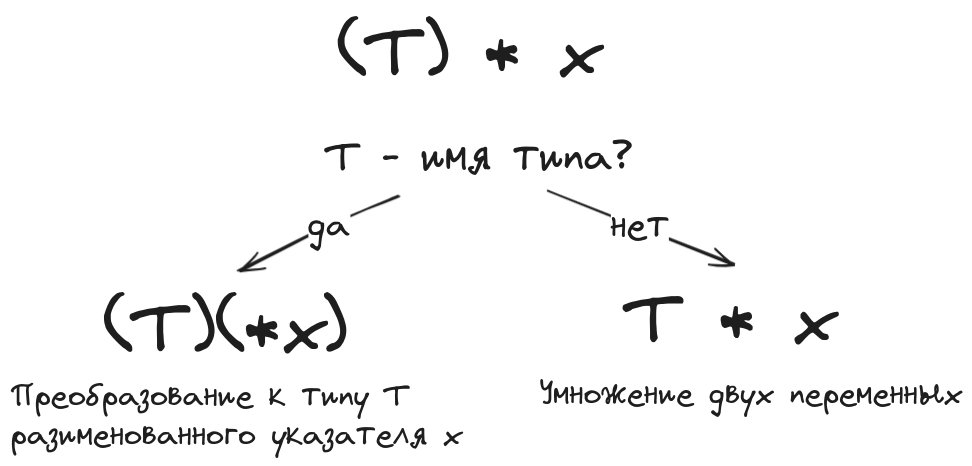
\includegraphics[width=\textwidth,height=\textheight,keepaspectratio]{gram-dep-diag.png}
    \centering
    \caption{Зависимость грамматики выражений Си от контекста}
    \label{parsing:gram-dep-diag}
\end{figure}
\FloatBarrier


Далее в Си есть понятие затенения(shadowing) имен. 
Следующий пример демонстрирует, что имя типа может быть затенено (использовался компилятор gcc):

\begin{lstlisting}[language=c, caption={Пример затенения имен}, label={parsing:name-shadowing-ex}]
typedef int Foo2;

void test_type_name() {
    int Foo2 = 3;
    int x;
    x = (Foo2) + x;
}
\end{lstlisting}

\verb|Foo2| внутри функции \verb|test_type_name| затеняет \verb|typedef| определение, и выражение \verb|(Foo2) + x| разбирается как сумма, 
а не приведение к типу \verb|Foo| и унарный плюс.

Так что для корректного разбора выражений языка Си, нужна система разрешения имен.

Данная система выполнена в виде стека таблиц символов(далее тип \verb|C_Environment|).
Внизу стека лежит глобальная таблица символов, где хранятся определения типов и функций. Далее по стеку идут локальные таблицы символов, соответствующие вложенным блокам кода(scopes).

\begin{lstlisting}[language=c, caption={Определения структур сивола и окружения}, label={parsing:env-struct}]
typedef str_t C_Symbol;
typedef hashmap_T(C_Symbol, C_SymbolData) C_SymbolTable;

struct_def(C_SymbolData, {
    C_Ast_Node *node;
    ...
})

typedef darr_T(C_SymbolTable *) C_Environment;
\end{lstlisting}

Для разрешения имени функция \verb|c_environment_get_sym_data| идет по стеку сверху вниз, проверяя принадлежит ли имя текущему блоку.
Так при определении нового имени в текущем блоке, оно перекроет имена находящиеся в нижележащих блоках. 

\begin{lstlisting}[language=c, caption={Определение функции разрешения имени символа}, label={parsing:get-sym-data-def}]
C_SymbolData NLB(*)
c_environment_get_sym_data(C_Environment env, C_Symbol sym) {
    C_SymbolData *data = nullptr;
    for (isize_t i = (isize_t)darr_len(env) - 1; i >= 0; i -= 1) {
        data = hashmap_get(**darr_get_T(C_SymbolTable *, env, i), &sym);
        if (data != nullptr) {
            break;
        }
    }
    return data;
}
\end{lstlisting}








\section{Функции грамматического разбора}

Рассмотрим самую внешнюю функцию грамматического разбора - функцию разбора единицы трансляции языка EC.
\begin{lstlisting}[language=c, caption={Функция разбора единицы трансляции}, label={parsing:ec-parse-tr-unit}]
ParsingError
ec_parse_translation_unit(ParserState *state, EC_Ast_TranslationUnit **out_tr_unit) {
    auto prev = parser_save(state);

    darr_t tr_unit_items;
    PARSER_ALLOC_HANDLE(darr_new_cap_in_T(EC_Ast_TrUnitItem *, 16, &state->ast_alloc, &tr_unit_items));

    EC_Ast_TrUnitItem *item = nullptr;
    while (parser_peek(state)->kind != C_TOKEN_KIND_EOF) {
        PARSER_ALLOC_HANDLE(darr_reserve_cap(&tr_unit_items, 1));
        if (parser_peek_punct_kind(state, C_PUNCT_AT)) {
            if (IS_ERR(ec_parse_at_directive(state, (EC_Ast_AtDirective **)&item))) {
                PARSING_NONE(state, &prev);
            }
        } else if (IS_ERR(c_parse_declaration(state, (C_Ast_Decl **)&item))) {
            PARSING_NONE(state, &prev);
        }

        *darr_get_unchecked_T(EC_Ast_TrUnitItem *, tr_unit_items, darr_len(tr_unit_items)) = item;
        tr_unit_items->len += 1;
    }

    make_node(state, out_tr_unit, EC_TR_UNIT, 
            .items = tr_unit_items,
            .span = parser_span_from_save(state, &prev),
        );

    return PARSING_ERROR(OK);
}
\end{lstlisting}



% \section{Идентификаторы и литералы}

% \beginminteddef{c}
% struct_def(C_Ast_Ident, {
%     C_AST_NODE_BASE

%     str_t name;
% })

% enum_def(C_Ast_LiteralKind, 
%     C_AST_LITERAL_KIND_INVALID,
%     C_AST_LITERAL_KIND_STRING,
%     C_AST_LITERAL_KIND_CHAR,
%     C_AST_LITERAL_KIND_NUMBER,
%     C_AST_LITERAL_KIND_COMPOUND,
% ) 
% \end{minted}

% \begin{itemize}
%     \item STRING, NUMBER, CHAR совпадают с соответствующими токенами
%     \item COMPOUND - составной литерал, например \verb|(str_t) {.ptr = nullptr, .byte_len = 0}|
% \end{itemize}

\clearpage
\section{Выражения}

Следующая диаграмма[\ref{parsing:expr-ast-diag}] иллюстрирует структуру AST для выражении языка Си: 

% \begin{tikzpicture}[
% roundnode/.style={ellipse, draw=black!60, fill=green!0, very thick, minimum size=7mm},
% squarednode/.style={rectangle, draw=red!60, fill=red!5, very thick, minimum size=5mm},
% ]
% %Nodes
% \node[roundnode]      (maintopic)                              {Expr};
% \node[roundnode]        (unop)       [below=of maintopic] {UnOp};
% \node[roundnode]      (binop)       [below=of maintopic] {BinOP};
% \node[roundnode]        (lowercircle)       [below=of maintopic] {4};

% %Lines
% \draw[->] (maintopic.north) -- (binop.south);
% \draw[->] (maintopic.north) -- (unop.south);
% % \draw[->] (uppercircle.south) -- (maintopic.north);
% % \draw[->] (rightsquare.south) .. controls +(down:7mm) and +(right:7mm) .. (lowercircle.east);
% \end{tikzpicture}


\begin{figure}[h!]
    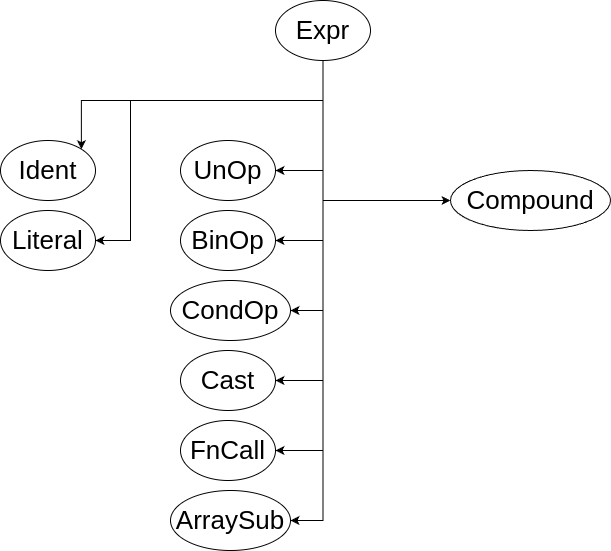
\includegraphics[width=\textwidth]{expr-ast.png}
    \centering
    \caption{AST выражения Си}
    \label{parsing:expr-ast-diag}
\end{figure}

% \begin{lstlisting}[language=c]
% enum_def(C_Ast_ExprKind, 
%     C_AST_EXPR_KIND_INVALID,
%     C_AST_EXPR_KIND_IDENT,
%     C_AST_EXPR_KIND_LITERAL,
%     C_AST_EXPR_KIND_UNOP,
%     C_AST_EXPR_KIND_BINOP,
%     C_AST_EXPR_KIND_CONDOP, // ?:
%     C_AST_EXPR_KIND_CAST,
%     C_AST_EXPR_KIND_FN_CALL,
%     C_AST_EXPR_KIND_ARRAY_,
%     C_AST_EXPR_KIND_COMPOUND, // expr, expr, ... expr
% )
% \end{lstlisting}

% \begin{itemize}
%   \item \verb|IDENT| - \verb|x|
%   \item \verb|LITERAL| - \verb|3|
%   \item \verb|UNOP| - \verb|-x|
%   \item \verb|BINOP| - \verb|x + y|
%   \item \verb|CONDOP| - \verb|x > y ? a : b|
%   \item \verb|CAST| - \verb|(T) expr|
%   \item \verb|FN_CALL| - \verb|f(e1, e2, e3)|
%   \item \verb|ARRAY_| - \verb|arr[x]|
%   \item \verb|COMPOUND| - \verb|e1, e2, e3|
% \end{itemize}

% % \beginminteddef{c}
% % \end{minted}

% \subsection{Разбор выражений}

Для разбора выражений используется парсер Пратта, который хорошо сочетается с разбором методом рекурсивного спуска.
Данный парсер использует таблицу приоритета и ассоциативности операторов. Данная таблица приведена в определениях[\ref{extras:c_defs}].

Операторы разделены на три группы: префиксные, инфиксные, постфиксные.
Отдельно обрабатывается тернарный условный оператор \verb|?:|.

Для каждого из этих групп есть функция, распознающая оператор по типу с ограничением по приоритету.

\begin{lstlisting}[language=c, caption={Функции разбора операторов}, label={parsing:expr:parse-op-headers}]
ParsingError
c_parse_expr_op_infix_prec_rb(ParserState *state, C_Ast_ExprBinOp **out_binop, u8_t max_precedence, bool is_strict_precedence);
ParsingError
c_parse_expr_op_prefix_prec_rb(ParserState *state, C_Ast_ExprUnOp **out_unop, u8_t max_precedence, bool is_strict_precedence);
ParsingError
c_parse_expr_op_postfix_prec_rb(ParserState *state, C_Ast_ExprUnOp **out_unop, u8_t max_precedence);
ParsingError
c_parse_expr_op_tern_cond_prec_rb(ParserState *state, C_Ast_ExprCondOp **out_tern, u8_t max_precedence, bool is_strict_precedence);
\end{lstlisting}

Замечание: числовое значение приоритета идет(возрастает) в порядке убывания приоритета[\cite{cppref_op_prec}].

Так например \verb|c_parse_expr_op_infix_prec_rb| проверяет принадлежит ли пунктуатор множеству инфиксных операторов,
затем если приоритет оператора ниже минимального приоритета, то функция выходит с ошибкой, 
если приоритет совпадает с минимальным, то проверяется ассоциативность, если оператор группируется слева на право, то функция выходит с ошибкой.
Также существует флаг \verb|STRICT_PRECEDENCE|, отсекающий случай равных приоритетов.

Следующие функции разбирают выражения, имплементацию их можно посмотреть в приложении[\ref{extras:parse_expr}].

\begin{lstlisting}[language=c, caption={Заголовки функции разбора выражений}, label={parsing:expr:parse-expr-headers}]
ParsingError
_c_parse_expr(ParserState *state, C_Ast_Expr **out_expr, u8_t max_precedence, C_ExprFlags flags);
ParsingError
c_parse_expr_assign(ParserState *state, C_Ast_Expr **out_expr);
ParsingError
c_parse_expr_cond(ParserState *state, C_Ast_Expr **out_expr);
ParsingError
c_parse_expr(ParserState *state, C_Ast_Expr **out_expr);
\end{lstlisting}


Графическое изображение AST выражения см. далее[\ref{pratt:right-lean-diag}] и [\ref{graphviz:expr}]

\section{Алгоритм парсера Пратта}
\label{pass:parsing:pratt}

Парсер Пратта использует комбинацию циклов и рекурсивных вызовов функций.
Есть хорошая статья, в которой приводится реализация данного парсера на языке Rust\cite{matklad_pratt_parsers}.

Парсер Пратта для инфиксных операторов упрощенно работает по следующему принципу: 

% \begin{lstlisting}[language=python, caption={Псевдокод алгоритма парсера Пратта}]
% def parse_expr(state, max_precedence, flags) -> expr, err:
%     left: Expr
    
% \end{lstlisting}

\begin{enumerate}
    \item Начало определения рекурсивной функции \verb|parse_expr|, 
    принимающей параметры состояния разбора \verb|state| и максимального значения порядка следования \verb|max_precedence|

    \begin{itemize}
        \item Пусть \verb|left: Expr| - переменная типа \verb|Expr|

        \item В \verb|left| записывается первый аргумент или выходим с ошибкой, если его нет или он является именем типа

        \item\label{pratt:alg:loop} Пока есть следующий за аргументом бинарный оператор, удовлетворяющий ограничениям порядка следования и ассоциативности:

        \begin{itemize}
            \item Разбираем оператор записываем в переменную \verb|op: Expr|

            \item\label{pratt:alg:rec-call} Разбираем правый операнд выражения рекурсивным вызовом функции \verb|parse_expr|, 
            со значением \verb|max_precedence| равным порядку следования оператора в переменной \verb|op|

            \item Записываем в \verb|left| значение переменной \verb|op|
        \end{itemize}
    \end{itemize}

    \item Конец определения функции \verb|parse_expr|
\end{enumerate}


Рекурсивные вызовы[\ref{pratt:alg:rec-call}] в алгоритме сами по себе разбирают цепочки операторов с убывающем номером порядка следования
(или одинаковым при условии ассоциативности справа на лево). 
Синтаксические деревья полученные после разбора таких операторов, являются наклоненными направо, как показано на диаграмме[\ref{pratt:right-lean-diag}].

Тогда как цикл[\ref{pratt:alg:loop}] в алгоритме сам по себе разбирает цепочки операторов с оставшимися после рекурсивного вызова номерами порядка следования, 
т.е. возрастающими или одинаковыми при условии ассоциативности слева на право. 
Синтаксические деревья полученные после разбора таких операторов, являются наклоненными налево, как показано на диаграмме[\ref{pratt:left-lean-diag}].


% \begin{figure}[h!]
%     \begin{figure}{.5\textwidth}
%         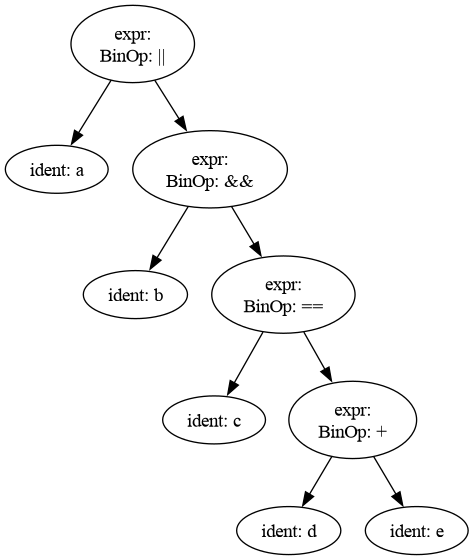
\includegraphics[width=.4\linewidth]{right-lean-diag.png}
%         \centering
%         \caption{AST цепочки операторов с убывающим номером порядка следования}
%         \label{pratt:right-lean-diag}
%     \end{figure}

%     \begin{figure}{.5\textwidth}
%         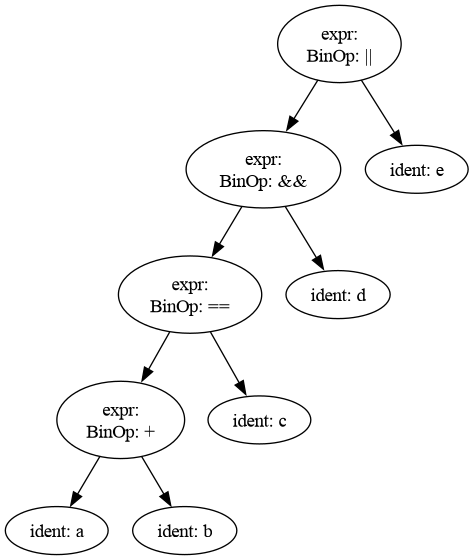
\includegraphics[width=.4\linewidth]{left-lean-diag.png}
%         \centering
%         \caption{AST цепочки операторов с возрастающим номером порядка следования}
%         \label{pratt:left-lean-diag}
%     \end{figure}
% \end{figure}

% \begin{figure}[h!]
%     \centering
%     \begin{minipage}{.5\textwidth}
%         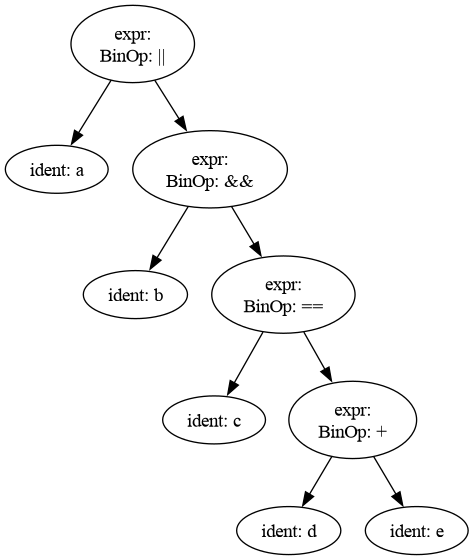
\includegraphics[width=.4\linewidth]{right-lean-diag.png}
%         \centering
%         \caption{AST цепочки операторов с убывающим номером порядка следования}
%         \label{pratt:right-lean-diag}
%     \end{minipage}
%     \begin{minipage}{.5\textwidth}
%         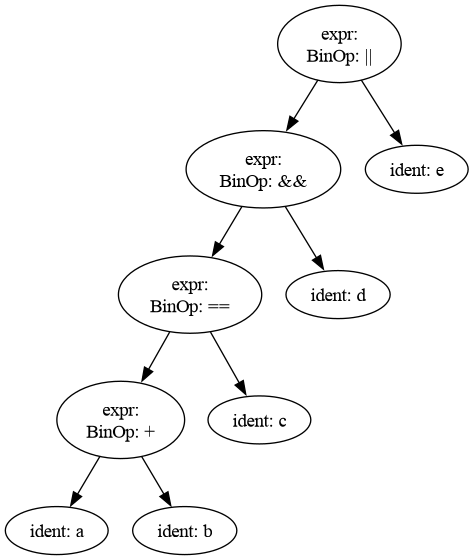
\includegraphics[width=.4\linewidth]{left-lean-diag.png}
%         \centering
%         \caption{AST цепочки операторов с возрастающим номером порядка следования}
%         \label{pratt:left-lean-diag}
%     \end{minipage}
% \end{figure}

\begin{figure}[h!]
    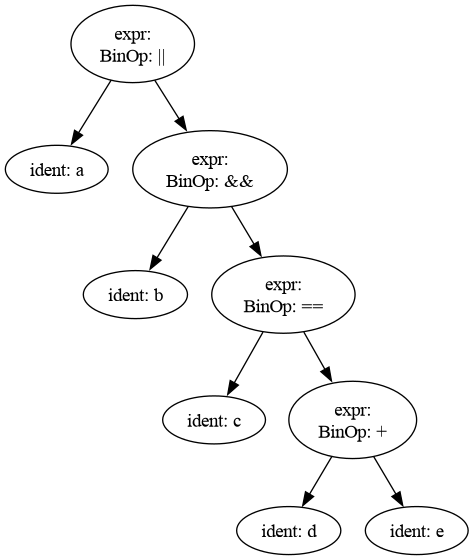
\includegraphics[width=.4\linewidth]{right-lean-diag.png}
    \centering
    \caption{AST цепочки операторов с убывающим номером порядка следования}
    \label{pratt:right-lean-diag}
\end{figure}
\begin{figure}[h!]
    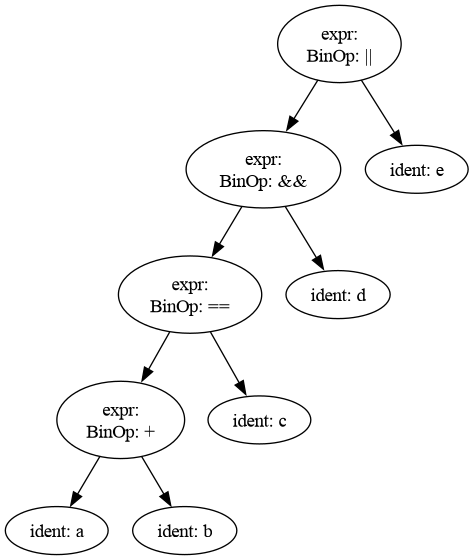
\includegraphics[width=.4\linewidth]{left-lean-diag.png}
    \centering
    \caption{AST цепочки операторов с возрастающим номером порядка следования}
    \label{pratt:left-lean-diag}
\end{figure}

\FloatBarrier


Комбинируя два этих подхода получаем всевозможные синтаксические деревья для выражений.

Подробнее данный алгоритм можно посмотреть в реализации функции \verb|_c_parse_expr| в приложении[\ref{extras:parse_expr}].



% \section{Определения}

% Виды нод типов:
% \beginminteddef{c}
% enum_def(C_Ast_TypeKind, 
%     C_AST_TYPE_KIND_INVALID,
%     C_AST_TYPE_KIND_IDENT,
%     C_AST_TYPE_KIND_POINTER,
%     C_AST_TYPE_KIND_ARRAY,
%     C_AST_TYPE_KIND_FUNCTION,
%     C_AST_TYPE_KIND_STRUCT,
%     C_AST_TYPE_KIND_UNION,
%     C_AST_TYPE_KIND_ENUM
% )
% \end{minted}

% Виды нод определений:
% \beginminteddef{c}
%     C_AST_DECL_KIND_INVALID,
%     C_AST_DECL_KIND_EMPTY, // ;;
%     C_AST_DECL_KIND_TYPE_DECL, // `struct(enum, union) A {};`
%     C_AST_DECL_KIND_VARIABLE, //  `struct A {} a;`, `int (*foo_p)(void), foo(void);`
%     C_AST_DECL_KIND_FN_DEF, // `int foo(void) {}`
%     C_AST_DECL_KIND_TYPEDEF, // typedef int Foo(void), Arr[3];
% \end{minted}


% Следующие функции разбирают определения, имплементацию их можно посмотреть в приложении[\ref{extras:parse_decl}]
% \beginminteddef{c}
% ParsingError
% c_parse_declarator(ParserState *state, C_Ast_Type **decl_ty_head, C_Ast_Type **decl_ty_leaf, C_Ast_Ident **decl_name);
% ParsingError
% c_parse_direct_declarator(ParserState *state, C_Ast_Type **decl_ty_head, C_Ast_Type **decl_ty_leaf, C_Ast_Ident **decl_name);
% ParsingError
% c_parse_record(ParserState *state, C_Ast_TypeKind struct_or_union_kind, C_Ast_TypeRecord **out_rec);
% ParsingError
% c_parse_type_specifier(ParserState *state, C_Ast_Type **out_ty);
% ParsingError
% c_parse_declaration(ParserState *state, C_Ast_Decl **out_decl);
% \end{minted}

% Функции \verb|c_parse_declarator|, \verb|c_parse_direct_declarator| взаимно рекурсивны, часть их задачи является разбор типов указателей массивов и функций, т.е. выражений вида:
% \mint{c}|int (*(*x)[3])(int a)| 

% Пример визуализации AST для такого определения см. далее[\ref{graphviz:decl}]


% \section{Утверждения}

% Виды утверждений:
% \beginminteddef{c}
% enum_def(C_Ast_StmtKind, 
%     C_AST_STMT_KIND_INVALID,
%     C_AST_STMT_KIND_EXPR,

%     C_AST_STMT_KIND_IF,
%     C_AST_STMT_KIND_SWITCH,

%     C_AST_STMT_KIND_LABEL,
%     C_AST_STMT_KIND_CASE,
%     C_AST_STMT_KIND_DEFAULT,

%     C_AST_STMT_KIND_FOR,
%     C_AST_STMT_KIND_WHILE,
%     C_AST_STMT_KIND_DO_WHILE,

%     C_AST_STMT_KIND_GOTO,
%     C_AST_STMT_KIND_CONTINUE,
%     C_AST_STMT_KIND_BREAK,
%     C_AST_STMT_KIND_RETURN,

%     C_AST_STMT_KIND_COMPOUND
% )
% \end{minted}

% \verb|EXPR| - любое выражение оконченное символом \verb|';'| \\
% \verb|COMPOUND| - блок(scope) утверждений, вида

% \beginminteddef{c}
% {
%   // ...
% }
% \end{minted}

% Элементом такого блока является утверждение или определение:
% \beginminteddef{c}
% struct_def(C_Ast_BlockItem, {
%     union {
%     struct {
%         C_AST_NODE_BASE
%     };
%         C_Ast_Decl decl;
%         C_Ast_Stmt stmt;
%     };
    
% })
% \end{minted}


% Остальные виды утверждений очевидно определяются по названию.


% Следующие функции разбирают утверждения, имплементацию их можно посмотреть в приложении[\ref{extras:parse_decl}]
% \beginminteddef{c}
% INLINE
% ParsingError
% c_parse_stmt_expr(ParserState *state, C_Ast_StmtExpr **out_stmt_expr);
% ParsingError
% c_parse_block(ParserState *state, C_SymbolTable *scope, darr_T(C_Ast_BlockItem *) *out_items);
% ParsingError
% c_parse_stmt(ParserState *state, C_Ast_Stmt **out_stmt);
% \end{minted}

% Функция \verb|c_parse_block| добавляет новое пространство имен в \verb|ParserState::env| и заполняет его.


% \section{Единица трансляции}

% \verb|C_Ast_TranslationUnit| - AST элемент единица трансляции разбирается схоже с составные утверждением (функция \verb|c_parse_block|),
% однако элементами единицы трансляции являются только определения.

% Следующая функция разбирает единицу трансляции и является самой общей функцией, с нее начинается грамматический разбор.
% \beginminteddef{c}
% ParsingError
% c_parse_translation_unit(ParserState *state, C_Ast_TranslationUnit **out_tr_unit);
% \end{minted}
% Ее реализация приведена в приложении[\ref{extras:parse_tr_unit}].

% Все выше перечисленное организованно в виде прохода:
% \beginminteddef{c}
% bool
% c_translation_unit_parse(C_TranslationUnitData *self) {
%     ASSERT_OK(arena_init(&self->ast_arena, darr_len(self->tokens), ctx_global_alloc));

%     ParserState pstate;

%     _translation_unit_parser_init(self, &pstate);

%         if (IS_ERR(c_parse_translation_unit(&pstate, &self->tr_unit))) {
%         parser_error_print(&pstate);
%         _translation_unit_parser_deinit(&pstate);
%         return false;
%     }

%     _translation_unit_parser_deinit(&pstate);
%     return true;
% }
% \end{minted}


Таким образом после этапа грамматического разбора мы получаем абстрактное синтаксическое дерево, которое может использовать в дальнейшей работе.

По итогам данной главы были рассмотрены основные этапы и методы синтаксического анализа.
% \clearpage
\chapter{ТРАНСЛЯЦИЯ AST}

Трансляция AST осуществляется с помощью обхода дерева в глубину, что иллюстрирует следующее изображение[\ref{pass:compile-c:dfs-diag}]:

\begin{figure}[h!]
    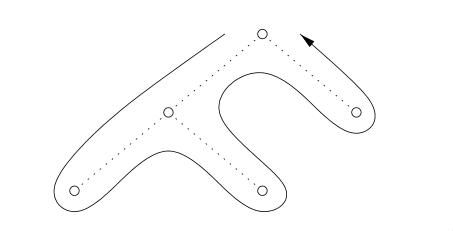
\includegraphics[width=0.6\linewidth]{tree-dfs.png}
    \centering
    \caption{Обход в глубину}
    \label{pass:compile-c:dfs-diag}
\end{figure}
\FloatBarrier

\section{Визуализация AST: Трансляция в dot}
\label{pass:compile-dot}

Можно визуализировать AST путем трансляции его к языку \textquote{dot} утилиты graphviz.
Трансляция выполнена в виде рекурсивного обхода AST аналогично трансляции в Си рассмотренной ранее[\ref{pass:compile-c}].
Примеры функции трансляции приведены [\ref{extras:compile-graphviz}].

Организуем код в виде функции единицы трансляции и тестируем:

\lstinputlisting[language={c},caption={Код теста визуализации}]{listings/translation/ast_vis/graphviz_test.c}

% \clearpage
Из входного файла \verb|ex_gv.c|:

\begin{lstlisting}[language=c, caption={ex\_gv.c}]
struct S {
    int x;
    Foo *foo;
};
\end{lstlisting}

Получаем файл \verb|ex_out.dot|:

\lstinputlisting[language={bash},caption={ex\_out.dot}]{listings/translation/ast_vis/ex_out.dot}
\clearpage
Применяем к нему движок dot фреймворка graphviz
\begin{lstlisting}[language=bash]
dot -Tpng sandbox/ex_out.dot -o build/ex_out.png
\end{lstlisting}

Получаем схему[\ref{graphviz:struct}]:

\begin{figure}[h!]
    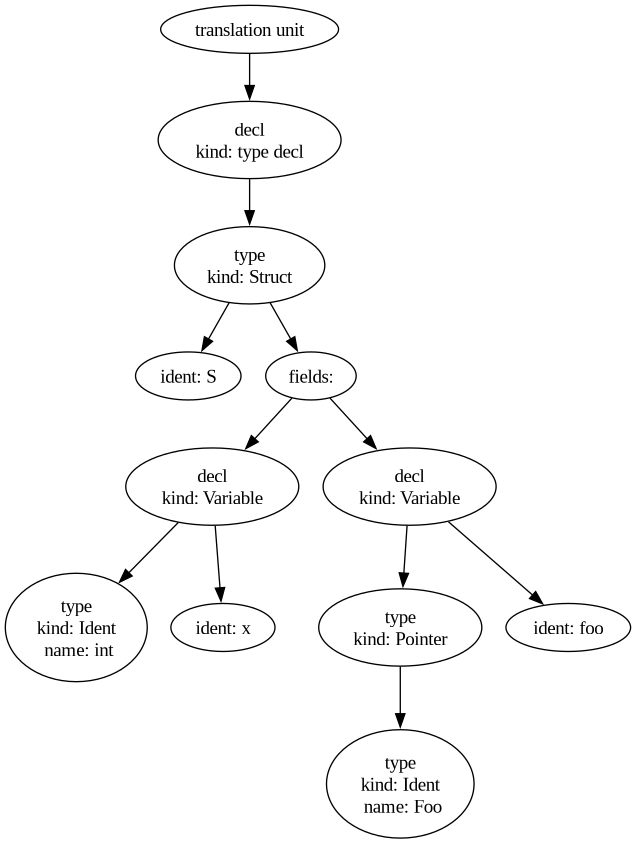
\includegraphics[width=\textwidth,height=0.7\textheight,keepaspectratio]{ex_out.png}
    \centering
    \caption{Синтаксическое дерево программы Си}
    \label{graphviz:struct}
\end{figure}

% \begin{figure}
%     \centering
%     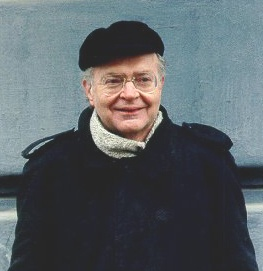
\includegraphics[width=0.6\linewidth]{images/knuth}
%     \caption{Knuth}
%     \label{fig:my_label4}
% \end{figure}

\clearpage
Теперь визуализируем следующее сложное определение переменных Си, где определения для трех переменных совмещены в одно.
\begin{lstlisting}[language=c]
int *(*x())[], y, *z;
\end{lstlisting}

После трансляции данного определения в язык dot с последующей компиляцией
получаем следующую схему AST выражения[\ref{graphviz:decl}]:

\begin{figure}[h!]
    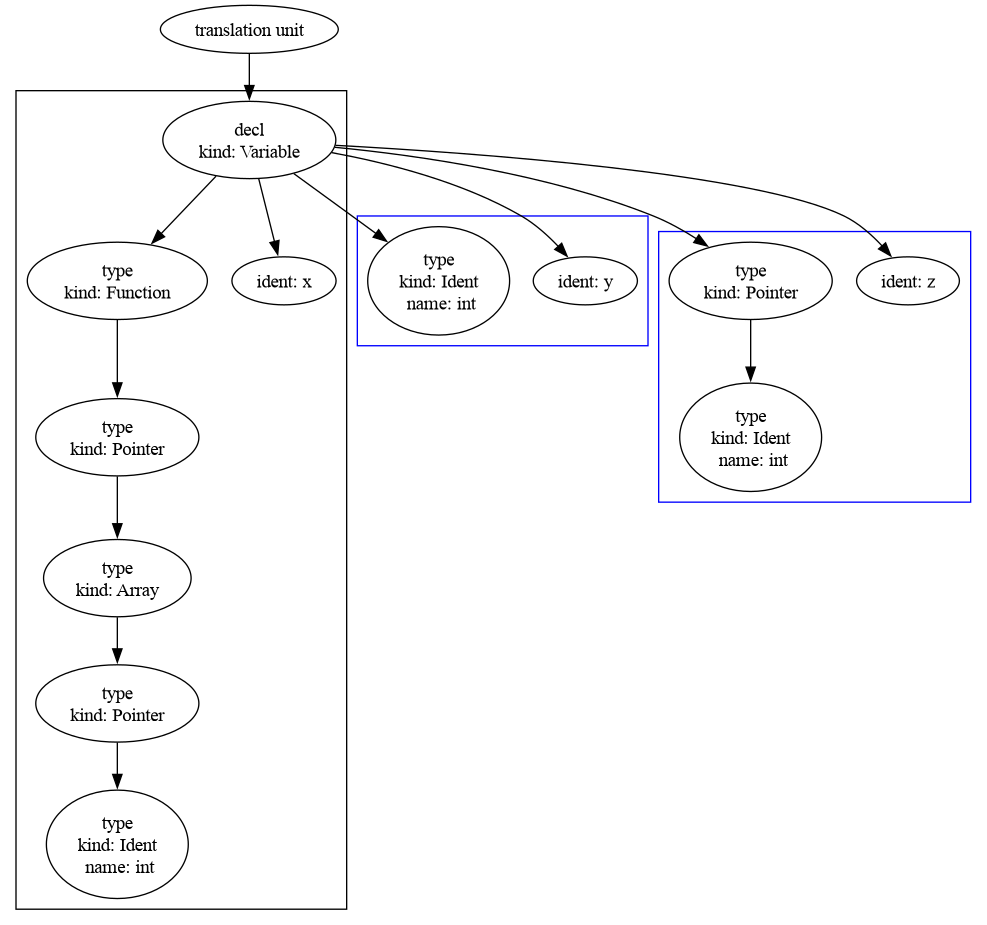
\includegraphics[width=\textwidth,height=\textheight,keepaspectratio]{ty_out.png}
    \centering
    \caption{AST сложного определения переменных Си}
    \label{graphviz:decl}
\end{figure}

\clearpage
Аналогично визуализируем выражение.
\begin{lstlisting}[language=c]
x = (a = a1) && b == c || d
\end{lstlisting}

После трансляции данного определения в язык dot с последующей компиляцией
получаем следующую схему AST выражения[\ref{graphviz:expr}]:
\begin{figure}[h!]
    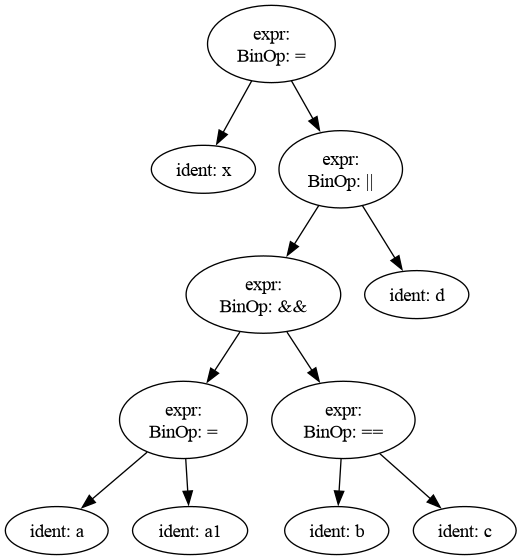
\includegraphics[width=0.8\textwidth]{expr_out.png}
    \centering
    \caption{AST выражения Си}
    \label{graphviz:expr}
\end{figure}

Таким образом данный функционал позволяет повысить наглядность структуры AST, что использовалось при отладке парсера, в частности парсера выражений, где можно ошибиться с порядком следования операторов.








\section{Трансляция AST в язык Си}
\label{pass:compile-c}


Рассмотрим как происходит процесс трансляции в язык Си. За это отвечает проход, выполненный в виде функции \hfill\break\verb|ec_translation_unit_ast_compile_c|.

\begin{lstlisting}[language=c, caption={Проход трансляции в язык Си}, label={pass:compile-c:compile-c-impl}]
void
ec_translation_unit_ast_compile_c(C_TranslationUnitData *self, StreamWriter *dst_sw) {
    auto fmt = string_formatter_default(dst_sw);
    ASSERT_OK(ec_ast_translation_unit_compile_c_fmt((EC_Ast_TranslationUnit *)self->tr_unit, &fmt, nullptr));
    ASSERT_OK(string_formatter_done(&fmt));
}
\end{lstlisting}

% Все, что данная функция делает это создает объект типа \verb|StringFormatter| с помощью выходного потока \verb|dst_sw| и передает его в основную функцию 
% трансляции \verb|ec_ast_translation_unit_compile_c_fmt|.

Данная функция является оберткой над основной функцией \newline \verb|ec_ast_translation_unit_compile_c_fmt|, применяющая интерфейс типа \verb|StringFormatter|.

Код основной функции привожу далее[\ref{pass:compile-c:compile-c-fmt-impl}]:

\begin{lstlisting}[language=c, caption={Функция трансляции типа Единицы Трансляции}, label={pass:compile-c:compile-c-fmt-impl}]
FmtError
ec_ast_translation_unit_compile_c_fmt(EC_Ast_TranslationUnit *tr_unit, StringFormatter *fmt, void *_) {
    auto items = tr_unit->items;
    for_in_range(i, 0, darr_len(items)) {
        auto item = *darr_get_T(EC_Ast_TrUnitItem *, items, i);
        if (item->kind == C_AST_NODE_KIND_DECL) {
            auto decl = (C_Ast_Decl *)item;
            if (decl->decl_kind == C_AST_DECL_KIND_EMPTY) {
                continue;
            }
            TRY(c_ast_decl_unparse_fmt(decl, fmt, nullptr));
            TRY(string_formatter_write(fmt, S("\n\n")));
        } else if (item->kind == C_AST_NODE_KIND_AT_DIRECTIVE) {
            auto dir = (EC_Ast_AtDirective *)item;
            TRY(ec_interpret_post_at_directive_fmt(dir, fmt, nullptr));
        } else {
            unreacheble();
        }
    }

    return FMT_ERROR(OK);
}
\end{lstlisting}


Данная функция в цикле проходится по всем корневым определениям и оставшимся директивам(в текущем прототипе только \verb|@post_include|),
печатая их с помощью типа \verb|StringFormatter| в выходной поток.

Трансляция определений производится обходом AST в глубину с помощью взаимно рекурсивных функций, заголовки которых приведены ниже[\ref{pass:compile-c:unparse-headers}]:

\begin{lstlisting}[language=c, caption={Заголовки функций трансляции AST в язык Си}, label={pass:compile-c:unparse-headers}]
FmtError
c_ast_ident_unparse_fmt(C_Ast_Ident *ident, StringFormatter *fmt, void *_);
FmtError
c_ast_expr_unparse_fmt(C_Ast_Expr *expr, StringFormatter *fmt, bool force_parens);
FmtError
c_ast_decl_unparse_fmt(C_Ast_Decl *decl, StringFormatter *fmt, void *_);
FmtError
c_ast_record_unparse_fmt(C_Ast_TypeRecord *record, StringFormatter *fmt, void *_);
FmtError
c_ast_struct_unparse_fmt(C_Ast_TypeStruct *_struct, StringFormatter *fmt, void *_);
FmtError
c_ast_union_unparse_fmt(C_Ast_TypeUnion *_union, StringFormatter *fmt, void *_);
FmtError
c_ast_type_unparse_fmt(C_Ast_Type *ty, StringFormatter *fmt, void *var_name, bool discard_leaf);
\end{lstlisting}

Реализация некоторых из них приведена в приложении[\ref{extras:unparse}].

Данные функции принимают элемент AST, объект типа \verb|StringFormatter| и дополнительные параметры.
Данный интерфейс позволяет производить трансляцию в любой абстрактный поток вывода, находящийся в форматоре \verb|fmt|.



\verb|@post_include| директивы интерпретируются следующей функцией[\ref{pass:compile-c:interpret-impl}]:

\begin{lstlisting}[language=c, caption={Функция трансляции директив}, label={pass:compile-c:interpret-impl}]
FmtError
ec_interpret_post_at_directive_fmt(EC_Ast_AtDirective *dir, StringFormatter *fmt, void *) {
    auto name = dir->name->name;
    if (str_eq(name, S("post_include"))) {
        ASSERT(dir->args && darr_len(dir->args) > 0);
        for_in_range(i, 0, darr_len(dir->args)) {
            auto arg = *darr_get_T(C_Ast_Literal *, dir->args, i);
            ASSERT(arg->lit_kind == C_AST_LITERAL_KIND_STRING);
            TRY(string_formatter_write_fmt(fmt, S("#include \"%s\"\n"), arg->l_str.t_str_lit->str));
        }
    } else {
        unreacheble();
    }

    return FMT_ERROR(OK);
}
\end{lstlisting}

Данная функций для каждого своего аргумента, который должен быть приведен в виде строкового литерала, печатает аналогичную \verb|#include| директиву препроцессора Си.

Таким образом производится трансляция AST в язык Си.

% Входной файл \verb|ex.c|
% \begin{code}
%   \inputminted[breaklines=true, xleftmargin=1em, linenos, frame=single,
%   framesep=10pt, fontsize=\footnotesize]
%   {c}{listings/translation/unparse/ex.c}
%   \label{ex.c}
% \end{code}

% Выходной файл \verb|ex\_out.c|
% \begin{code}
%   \inputminted[breaklines=true, xleftmargin=1em, linenos, frame=single,
%   framesep=10pt, fontsize=\footnotesize]
%   {c}{listings/translation/unparse/ex_out.c}
%   \label{ex_out.c}
% \end{code}

Итак на данном этапе был разобран функционал библиотеки позволяющий преобразовывать текст программы к синтаксическому дереву и обратно, 
т.е. выполнять сериализацию/десериализацию AST. Если сейчас последовательно применить лексический, грамматический разборы и затем транслировать дерево обратно в Си, то 
получатся практически идентичные файлы за исключением, может быть, кол-ва пробелов и переносов строк. 
Теперь вставленные между стадиями разбора и трансляции проходы будут отображены в выходном файле.
Данные этапы(проходы) модификации AST будут рассмотрены в следующей главе.

\clearpage
\section{Упорядочивание определений}
\label{pass:ordering}

На данном этапе у нас есть массив определений(и возможно оставшихся директив), 
который нам надо преобразовать так, чтобы его смог скомпилировать компилятор языка Си.

Для этого нам нужно расположить все определения следующим образом:

Сначала идут оставшиеся директивы, например:
\begin{lstlisting}[language=c]
@post_include("demo.ec")    
\end{lstlisting}

Затем идут предекларации типов, например:
\begin{lstlisting}[language=c]
struct Foo;
typedef struct Foo Foo;
\end{lstlisting}

Затем сами типы, упорядоченные топологически по графу зависимостей между ними, например:
\begin{lstlisting}[language=c]
struct C {
    B *bp;
};
struct B {
    A *ap;
    C c;
};
struct A {
    B b;
};
\end{lstlisting}

Далее идут определения глобальных переменных, например:
\begin{lstlisting}[language=c]
int g_x;
\end{lstlisting}

Далее заголовки функций, например:
\begin{lstlisting}[language=c]
void bar();
void foo(int x);
\end{lstlisting}

В конце идут определения функций, например:
\begin{lstlisting}[language=c]
void bar() {
    foo(g_x);
}
void foo(int x) {
    print_fmt(S("x: %d\n"), x);
}
\end{lstlisting}

Заметим, что определения типов это единственное место, где нужно делать топологическую сортировку, 
т.к. определения функций зависят только от имен других функций, типов, глобальных переменных, которые идут ранее в порядке декларации.

Для того, чтобы упорядочить определения таким образом мы сначала проходим весь список определений в цикле, распределяя их по группам:
определения переменных, определения функций и те что надо отсортировать. Определения переменных и функций хранятся в массивах, сортируемые хранятся сразу на узлах графа в хеш-таблице.
Оставшиеся директивы сразу записываются в выходной массив, т.к идут первыми. Предекларации составных типов игнорируются.
Для сортируемых рекурсивным обходом его AST формируются хеш-множества зависимостей для сортируемого элемента, данные множества добавляются в соответствующие хеш-таблицы графов.
Замечание: собираются только \textquote{сильные} зависимости т.е. те, где тип приведен без указателя.

Итак в процессе вывода зависимостей строятся два графа сам граф зависимостей \verb|deps_table| и его копия с развернутыми ребрами \verb|f_deps_table|.
Далее два графа сливаются в один \verb|deps_table|.
Для каждого узла переменная \verb|in_deg| устанавливается равной кол-ву зависимостей данного узла.
Формируется массив узлов, для которых переменна \verb|in_deg| равна 0.
После чего запускается алгоритм топологической сортировки[\ref{pass:ordering:topsort}].

Далее в выходной массив из отсортированного массива типов генерируются предекларации, что нужно для разрешения зависимостей по указателю(в моей терминологии \textquote{слабых}).
Далее из отсортированного пишутся сами определения типов.
Затем пишутся определения переменных.
Затем из массива определений функций генерируются их заголовки.
Затем пишутся сами определения функции.

\subsection{Алгоритм топологической сортировки}
\label{pass:ordering:topsort}

Для топологической сортировки определений используется алгоритм Кана. Данный алгоритм топологически сортирует направленный ациклический граф
Данный алгоритм требует входные данные: 
\begin{itemize}
\item сам направленный ациклический граф $G$
\item множество начальных элементов графа $G$ - те элементы, у которых нет предков, т.е. их входная степень равна нулю
\item множество переменных входных степеней элементов графа $G$ - изначально значение каждой переменной равно значению кол-ва предков для соответствующей вершины или входной степени этой вершины
\item выходной массив $O$, который изначально пустой
\end{itemize}

Алгоритм использует стек в процессе своей работы, в моей реализации подразумевается, что на стеке оказываются элементы у которых текущая входная степень равна нулю.

\begin{itemize}
    \item множество начальных элементов кладется на стек в произвольном порядке

    \item пока стек не пуст выполняется:
    \begin{itemize}
        \item со стека снимается элемент $E$
        \item элемент $E$ добавляется в выходной массив $O$
        \item для любого соседнего элемента $D$ вершины $E$ выполняется: 
        \begin{itemize}
            \item понизь текущую степень $D$ на 1
            \item если текущая степень $D$ равна 0, добавь $D$ на стек
        \end{itemize}
    \end{itemize}

    \item сравниваются величины $\abs{G}$ $\abs{O}$, если они различаются, значит в графе присутствует цикл и алгоритм возвращает ошибку
\end{itemize}

Привожу реализацию[\ref{pass:ordering:kahn-impl}] данного алгоритма для сортировки символов по зависимостям между ними:

\begin{lstlisting}[language=c, caption={Реализация алгоритма Кана}, label={pass:ordering:kahn-impl}]
bool
symbol_topsort(darr_T(C_Symbol) initials, C_SymbolTable table, darr_T(C_Symbol) *out_sorted, Allocator *alloc) {
    darr_t sorted;
    ASSERT_OK(darr_new_cap_in_T(C_Symbol, hashmap_len(table), alloc, &sorted));

    darr_t stack = initials;

    while (darr_len(stack) > 0) {
        C_Symbol cur = *darr_get_iT(C_Symbol, stack, -1);
        darr_pop(&stack);
        usize_t *cur_in_deg = &hashmap_get_T(C_SymbolData, table, &cur)->in_deg;
        ASSERT(*cur_in_deg == 0);

        hashset_T(C_Symbol) f_deps = hashmap_get_T(C_SymbolData, table, &cur)->f_deps;
        for_in_range(i, 0ul, hashset_len(f_deps)) {
            C_Symbol f_dep = *slice_get_T(C_Symbol, &hashset_values_raw(f_deps), i);
            usize_t *f_dep_in_deg = &hashmap_get_T(C_SymbolData, table, &f_dep)->in_deg;
            ASSERT(*f_dep_in_deg > 0);
            *f_dep_in_deg -= 1;
            if (*f_dep_in_deg == 0) {
                ASSERT_OK(darr_push(&stack, &f_dep));
            }
        }

        ASSERT_OK(darr_push(&sorted, &cur));
    }

    if (darr_len(sorted) != hashmap_len(table)) {
        return false;
    }

    *out_sorted = sorted;

    return true;
}
\end{lstlisting}

Реализация данного алгоритма принимает динамический массив начальных символов, граф в виде хеш-таблицы, элементы которой хранят соседей элемента графа в виде хеш-множества, а также количество предков данного элемента.

% Код данного прохода представлен в приложении[\ref{extras:pass:ordering}]

\clearpage
\section{Система макросов}
\label{pass:macros}

Язык EC содержит систему макро-функций, предоставляющую удобный интерфейс для метапрограммирования.
Принцип ее работы
Пользователь определяет свои макро-функции в отдельном модуле(файле), помечая их с помощью директив(на данный момент есть только \verb|@derive_macro|).
В основном файле пользователь помечает определения, которые хочет модифицировать с помощью соответствующих директив (на данный момент есть только \verb|@derive|).

Применение макросов идет в три этапа:
\begin{enumerate}
    \item Компиляция модуля с макросами в отдельной единице трансляции в качестве динамической библиотеки(данная библиотека связывается(линкуется) с основной библиотекой \verb|libec.so|). 
        Также на данном этапе выполняется сбор и регистрация имен макросов совместно с символами функций в базе компилятора. Подробнее[\ref{pass:macros:compile}]
    \item Динамическая подгрузка получившейся библиотеки с макросами методами операционной системы, разрешение символов макро-функций.  Подробнее[\ref{pass:macros:load}]
    \item Применение загруженных макро-функций к определениям, посредством интерпретации соответствующих директив.  Подробнее[\ref{pass:macros:apply}]
\end{enumerate}

Привожу диаграмму[\ref{pass:macros:diag}], иллюстрирующую данный процесс и его зависимости:
\begin{figure}[h!]
    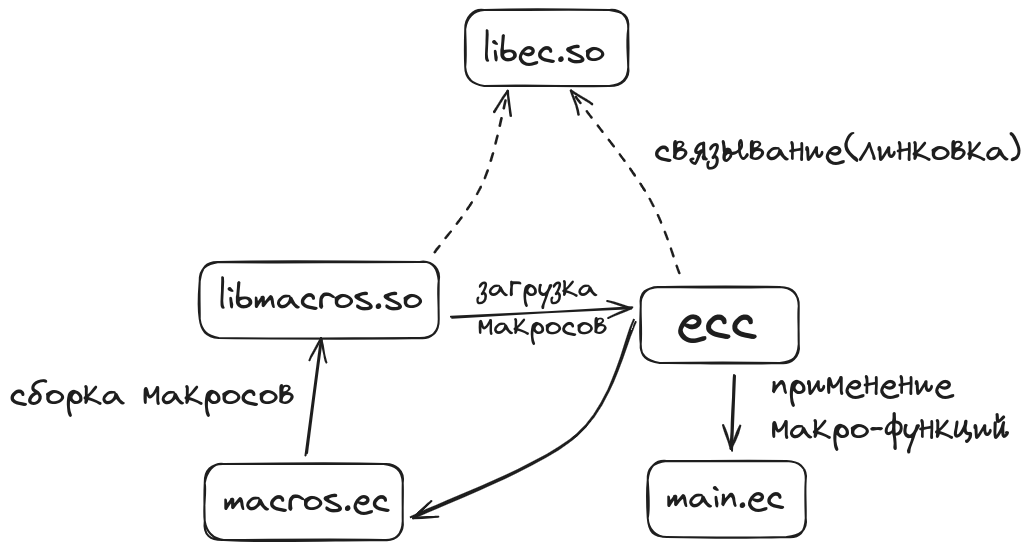
\includegraphics[width=\textwidth,height=\textheight,keepaspectratio]{macro-diag.png}
    \centering
    \caption{Процесс работы системы макро-функций}
    \label{pass:macros:diag}
\end{figure}
\FloatBarrier


% Термин символ в данном случае взят из терминологи линкера и означает упрощенно имя функции, переменной или в исходном коде языка(при условии, что компилятор не производит |name mangling|\cite{wiki:nm}).
% В случае языка Си, можно использовать это определение, т.к. он не производит изменения над именами функций(символами).
Термин символ в данном случае понимается как идентификатор, находящийся в таблице символов(аналогичной рассмотренной ранее[\ref{pass:parsing}]) линкера.
В случае языка Си это имя функции или переменной в исходном тексте программы, т.к. компилятор Си не производит изменение имен символов(\verb|name mangling|\cite{wiki-nm}).
В следующем листинге[\ref{pass:macros:macro-sym-diff}] имя символа - \verb|gen_dbg_fmt|, имя макро-функций, по которому она вызывается - \verb|DebugFormat|.

\begin{lstlisting}[language=c, caption={Заголовок функции gen\_dbg\_fmt}, label={pass:macros:macro-sym-diff}]
@derive_macro(DebugFormat)
ProcMacroError
gen_dbg_fmt(C_TranslationUnitData *data, C_Ast_Decl *decl, C_Ast_TranslationUnit **out_node);
\end{lstlisting}

Пример применения данной системы был рассмотрен выше[\ref{use-ex:code-gen}].


\section{Компиляция макросов}
\label{pass:macros:compile}
Рассмотрим процесс компиляции макросов подробнее.
Единица трансляции, в которой компилируются макросы отличается от обычной только тем, что в ней нет стадии применения макросов, 
что и понятно, ведь откуда их брать, если мы уже находимся в модуле, в котором все макро-функции должны быть. Все остальные стадии EC применяются.

Для этого этапа(прохода) в структуре \verb|TranslationUnitData| выделен блок[\ref{pass:macros:proc-macro-struct}].

\begin{lstlisting}[language=c, caption={Блок отвечающий за макро-функции}, label={pass:macros:proc-macro-struct}]
struct {
    hashmap_T(C_Symbol, EC_ProcMacroData) macros;
    void *lib; // handle from dlopen call

    void (*pm_init)();
    void (*pm_deinit)();
} proc_macro;
\end{lstlisting}

Данный блок содержит:
\begin{itemize}
    \item таблицу символов |macros|
    \item абстрактный указатель \verb|lib| на динамическую библиотеку, загружаемую в следующем параграфе[\ref{pass:macros:load}]
    \item указатели на динамически загружаемы функции инициализации и деинициализации динамически загружаемой библиотеки макросов
\end{itemize}


\begin{lstlisting}[language=c, caption={Структура содержащая информацию о символе макро-функции}, label={pass:macros:proc-macro-data-struct}]
enum_def(EC_ProcMacroKind,
    EC_PROC_MACRO_KIND_TRANSFORM,
    EC_PROC_MACRO_KIND_DERIVE,
    )

struct_def(EC_ProcMacroData, {
    EC_ProcMacroKind kind;
    str_t symbol_name;
    void *symbol;
})
\end{lstlisting}

Структура содержит информацию о:
\begin{itemize}
    \item типе символа \verb|kind|. На данный момент используется только тип \verb|DERIVE|
    \item имени символа \verb|symbol_name|
    \item указатель на машинный код символа в памяти \verb|symbol|
\end{itemize}
    
Привожу код функции отвечающей за компиляцию макросов:

\begin{lstlisting}[language=c, caption={Реализация функции компиляции макросов}, label={pass:macros:compile-impl}]
bool
ec_translation_unit_compile_macros(C_TranslationUnitData *self, C_BuildData *build_data) {
    if (self->string_arena.chunks == nullptr) {
        ASSERT_OK(arena_init(&self->string_arena, 4096, ctx_global_alloc));
    }

    C_TranslationUnitData macro_tr_unit;
    c_translation_unit_init(&macro_tr_unit, build_data->macro_path);
    ASSERT(c_translation_unit_lex(&macro_tr_unit));
    ASSERT(ec_translation_unit_parse(&macro_tr_unit));
    ASSERT(ec_translation_unit_collect_proc_macro_names(&macro_tr_unit, 
        arena_allocator(&self->string_arena), &self->proc_macro.macros));

    WITH_FILE(build_data->macro_tmp_c_path, "w", file, {
        OutputFileStream ofs;
        ASSERT_OK(file_sw(file, &ofs));
        auto sw = output_file_stream_stream_writer(&ofs);
        ec_translation_unit_ast_compile_c(&macro_tr_unit, &sw);
    })
    auto string_alloc = arena_allocator(&self->string_arena);
    String s;
    ASSERT_OK(string_new_cap_in(128, &string_alloc, &s));
    sprint_fmt(&s, S("%s %s -fPIC -shared -Wall -o %s -std=c2x -g -Wall -I. -I./lib -L./build -lec\0"), 
        build_data->cc_path, build_data->macro_tmp_c_path, build_data->macro_lib_path);
    s.byte_len -= 1;
    str_t build_cmd = string_to_str(&s);

    if (system((char *)build_cmd.ptr) != 0) { return false; }
    
    c_translation_unit_deinit(&macro_tr_unit);

    return true;
}
\end{lstlisting}

Как можно видеть сначала файл с макросами, полученный из \verb|build_data|, сначала преобразуется к AST, 
функциями \newline\verb|c_translation_unit_lex| и \verb|ec_translation_unit_parse|, 
рассмотренных ранее в соответствующих главах лексического[\ref{pass:lexing}] и грамматического разбора[\ref{pass:parsing}].

К полученному AST далее применяется проход \newline\verb|ec_translation_unit_collect_proc_macro_names|, 
который строит таблицу(заполняет) таблицу символов макро-функций[\ref{pass:macros:proc-macro-struct}], 
собирая имена макро-функций и имена символов, реализующие их.
Делает она это путем интерпретации директив(на данный момент только \verb|@derive_macro|).

После формирования таблицы символов для макро-функций, выполняется трансляция AST к коду языка Си функцией \newline\verb|ec_translation_unit_ast_compile_c|, 
разобранной ранее[\ref{pass:compile-c}]. Полученный код языка Си записывается в выходной промежуточный файл средствами типа \verb|OutputFileStream|.

Наконец промежуточный файл с кодом макро-функций на языке Си компилируется в динамическую библиотеку с помощью компилятора, 
предоставленного системой(в данном прототипе используется \verb|gcc|).
При этом происходит связывание(линковка) данной библиотеки макро-функций с библиотекой \verb|ec.so|.

Если на каком-то этапе выполнения некоторая подфункция вернет ошибку, то вся функция возвращается с ошибкой, возвращая |false|.

\section{Динамическая загрузка макросов}
\label{pass:macros:load}

После получения динамической библиотеки макро-функций(назовем \verb|libmacros.so|) выполняется динамическая загрузка библиотеки в виртуальную память процесса компилятора \verb|ecc|.
Далее привожу код[\ref{pass:macros:load-impl}] функции \verb|ec_translation_unit_load_macro_symbols|, выполняющей данную операцию. 

\begin{lstlisting}[language=c, caption={Реализация функции загрузки макросов}, label={pass:macros:load-impl}]
bool
ec_translation_unit_load_macro_symbols(C_TranslationUnitData *self, str_t libmacros_path) {
    ASSERT(self->proc_macro.macros != nullptr);

    auto string_alloc = arena_allocator(&self->string_arena);
    str_t lib_path;
    ASSERT_OK(str_null_terminate_in(libmacros_path, &string_alloc, &lib_path));

    void *lib = dlopen((char *)lib_path.ptr, RTLD_NOW);
    if (!lib) {
        fprintf(stderr, "dlopen failed: %s\n", dlerror());
        return false;
    }
    self->proc_macro.lib = lib;
    
    void *pm_init = dlsym(lib, "proc_macro_init");
    void *pm_deinit = dlsym(lib, "proc_macro_deinit");
    if (pm_init == nullptr) {
        fprintf(stderr, "dlsym for proc_macro_init failed: %s\n", dlerror());
        return false;
    }
    if (pm_deinit == nullptr) {
        fprintf(stderr, "dlsym for proc_macro_deinit failed: %s\n", dlerror());
        return false;
    }
    self->proc_macro.pm_init = pm_init;
    self->proc_macro.pm_deinit = pm_deinit;

    bool was_err = false;
    for_in_range(i, 0, hashmap_len(self->proc_macro.macros)) {
        auto val = slice_get_T(EC_ProcMacroData, &self->proc_macro.macros->values, i);
        // symbol_name is assumed to be null-terminated
        void *macro = dlsym(lib, (char *)val->symbol_name.ptr);
        if (macro == nullptr) {
            fprintf(stderr, "dlsym for %s failed: %s\n", (char *)val->symbol_name.ptr, dlerror());
            was_err = true;
        }
        val->symbol = macro;
    }
    if (was_err) {
        return false;
    }

    return true;
}
\end{lstlisting}

В настоящем прототипе загрузка выполняется средствами \verb|glibc| \verb|dlopen| и \verb|dlsym|.

Сначала символы динамической библиотеки подгружаются в память текущего процесса вызовом \verb|dlopen|(строка 9, \ref{pass:macros:load-impl}).
Далее разрешаются указатели на них вызовами \verb|dlsym|.

Подразумевается, что в библиотеке \verb|libmacros.so| присутствуют символы инициализации \verb|proc_macro_init| и деинициализации \verb|proc_macro_deinit| библиотеки макросов, 
на данный момент они определены в заголовочном файле \verb|proc_macro.h|(тот, что был в примере макро-функции вывода[\ref{use-ex:macro-file}]).
Их символы подгружаются в отведенный блок[\ref{pass:macros:proc-macro-struct}] структуры \verb|TranslationUnitData|.

Далее для каждой позиции в таблице символов макро-функций, полученной ранее на этапе компиляции макросов[\ref{pass:macros:compile}], 
разрешается указатель на соответствующий данному макросу символ.

Если какой-то символ не может быть разрешен, то функция данная функция[\ref{pass:macros:load-impl}] выдает ошибку.

\section{Применение макросов}
\label{pass:macros:apply}

Теперь, когда у нас есть таблица макро-функций с загруженными символами, мы можем применить макро-функции в коду основного модуля(единицы трансляции),
это делается после получения AST из кода основного модуля с помощью интерпретации директив.

Привожу код[\ref{pass:macros:apply-impl}] функции интерпретирующей директивы применения макро-функций(на данном этапе выполнена только директива \verb|@derive|):
\begin{lstlisting}[language=c, caption={Реализация функции применения макросов}, label={pass:macros:apply-impl}]
bool
ec_translation_unit_apply_proc_macros(C_TranslationUnitData *self) {
    ASSERT(self->proc_macro.macros);

    auto tr_unit = (EC_Ast_TranslationUnit *)self->tr_unit;
    if (darr_len(tr_unit->items) == 0) {
        return true;
    }
    auto ast_alloc = arena_allocator(&self->ast_arena);
    darr_t processed = nullptr;
    ASSERT_OK(darr_new_cap_in_T(EC_Ast_TrUnitItem *, darr_len(tr_unit->items), &ast_alloc, &processed));

    self->proc_macro.pm_init();

    for_in_range(i, 0, darr_len(tr_unit->items)) {
        auto item = *darr_get_T(EC_Ast_TrUnitItem *, tr_unit->items, i);
        if (item->kind == C_AST_NODE_KIND_DECL) {
            ASSERT_OK(darr_push(&processed, &item));
            continue;
        }
        ASSERT(item->kind == C_AST_NODE_KIND_AT_DIRECTIVE);

        auto name = item->at_directive.name->name;
        if (str_eq(name, S("derive"))) {
            if (i == darr_len(tr_unit->items)-1) {
                eprint_fmt(S("stray @derive macro invocation\n"));
                return false;
            }
            if (item->at_directive.args == nullptr || darr_len(item->at_directive.args) < 1) {
                eprint_fmt(S("@derive expects at least one argument\n"));
                return false;
            }

            auto next = *darr_get_T(EC_Ast_TrUnitItem *, tr_unit->items, i+1);
            if (next->kind != C_AST_NODE_KIND_DECL) {
                eprint_fmt(S("@derive expects declaration\n"));
                return false;
            }
            ASSERT_OK(darr_push(&processed, &next));
            for_in_range(j, 0, darr_len(item->at_directive.args)) {
                auto arg = *darr_get_T(C_Ast_Node *, item->at_directive.args, j);
                if (arg->kind != C_AST_NODE_KIND_IDENT) {
                    eprint_fmt(S("@derive expects arguments of type C_Ast_Ident\n"));
                    return false;
                }
                
                auto data = hashmap_get_T(EC_ProcMacroData, self->proc_macro.macros, &arg->ident.name);
                if (data == nullptr) {
                    eprint_fmt(S("there is no such macro %s\n"), arg->ident.name);
                    return false;
                }
                DeriveMacroFn *macro = (DeriveMacroFn *)data->symbol;
                C_Ast_TranslationUnit *res = nullptr;
                if (IS_ERR(macro(self, (C_Ast_Decl *)next, &res))) {
                    eprint_fmt(S("%s macro failed\n"), arg->ident.name);
                    return false;
                }
                ASSERT_OK(darr_append_slice(&processed, darr_slice_full(res->decls)));
            }
            i += 1;
        } else {
            ASSERT_OK(darr_push(&processed, &item));
            continue;
        }
    }

    self->proc_macro.pm_deinit();
    tr_unit->items = processed;
    return true;
}
\end{lstlisting}

При применении макро-функций первым делом надо инициализировать библиотеку макросов, делается это вызовом символа \verb|proc_macro_init|, который подгружен в указатель \verb|pm_init|.

После обработки новый список определений будет содержаться в динамическом массиве \verb|processed|.

Далее последовательно итерируем по списку корневых определений, определения без примененных к ним директив просто записываем в выходной массив.
При нахождении директивы интерпретируем ее следующим образом:
\begin{enumerate}
    \item проверяем существования определения, к которому должна быть применена директива
    \item проверяем, что в макро-функцию подавался хотя бы один аргумент
    \item проверяем, чтобы синтаксический тип аргументов, подаваемых в функцию, был \verb|C_Ast_Ident|
    \item загружаем соответствующий данному имени макроса символ из таблицы макросов \verb|proc_macro.macros| структуры \verb|TranslationUnitData|
    \item применяем полученный символ к последующему определению, получаем результат в виде типа \verb|C_Ast_TranslationUnit|
    \item добавляем определения из полученной AST единицы трансляции в выходной массив определений \verb|processed|
\end{enumerate}


По окончанию работы с библиотекой деинициализируем ее вызовом функции по указателю \verb|pm_deinit|.

Таким образом были рассмотрены все подсистемы, входящие в состав системы макро-функций.


% \subsubsection{Макросы}

% Для определений структур и энумераций используются следующие макросы:

% \beginminteddef{c}
% #define struct_decl(name) \
% typedef struct name name; \
% struct name; \

% #define enum_decl(name) \
% typedef enum name name; \
% enum name; \

% #define struct_def(name, fields) \
% typedef struct name name; \
% struct name fields; \

% #define enum_def(name, ...) \
% typedef enum name name; \
% enum name {__VA_ARGS__}; \
% \end{minted} 


% \subsubsection{Обработка ошибок}

% Ошибки кодируются как enum, например:

% \begin{listing}
% \caption{Ошибки Аллокатора}
% \beginminteddef{c}
% enum_def(AllocatorError,
%     ALLOCATOR_ERROR_OK,
%     ALLOCATOR_ERROR_MEM_ALLOC,
%     ALLOCATOR_ERROR_COUNT
% )
% #define ALLOCATOR_ERROR(ERR) ((AllocatorError)ALLOCATOR_ERROR_##ERR)
% \end{minted}
% \end{listing}

% Значение OK кодируется как 0, остальные значения кодируются положительными числами.

% Для обработки ошибок используются следующие макросы:
% % \begin{minted}[linenos, frame=single]{c}
% \beginminteddef{c}
% #define IS_OK(e) ({ \
%     auto _r = (e); \
%     *(int *)&(_r) == 0; \
%     })
% #define IS_ERR(e) ({ \
%     auto _r = (e); \
%     *(int *)&(_r) != 0; \
%     })
% #define TRY(expr) { \
%     auto _e_ = (expr); \
%     if (IS_ERR(_e_)) { \
%         return _e_; \
%     } \
%   }
% #define ASSERT(expr) \
%     if (!(expr)) { \
%         fprintf(stderr, "ASSERT at %s:%d:\n", __FILE__, __LINE__); \
%         panic(); \
%     } 
% #define ASSERTM(expr, msg) { \
%     if (!(expr)) { \
%         fprintf(stderr, "ASSERTM: %*s\nat %s:%d:\n", (int)(sizeof(msg)-1), msg, __FILE__, __LINE__); \
%         panic(); \
%     } \
% }
% #define ASSERT_OK(expr) { \
%     auto _e_ = (expr); \
%     if (IS_ERR(_e_)) { \
%         fprintf(stderr, "ASSERT_OK at %s:%d:\n", __FILE__, __LINE__); \
%         panic(); \
%     } \
% }
% \end{minted} 

% \verb|IS_OK|, \verb|IS_ERR| - проверяют была ли ошибка

% \verb|TRY| - если была ошибка верни ошибку из текущей функции 

% \verb|ASSERT_OK| - если была ошибка, критическое завершение программы 

% \subsubsection{Контекст}
% Используется глобальный контекст, уникальный для каждого потока:

% \beginminteddef{c}
% __thread struct {
%     Allocator global_alloc;

%     Arena imm_str_arena;
%     Allocator imm_str_alloc;
%     slice_T(u8_t) dump_buffer;

%     void (*raise)(Error);

%     StreamWriter stdout_sw;
%     StreamWriter stderr_sw;
% } g_ctx;
% \end{minted} 

% \subsubsection{Аллокатор}

% Вдохновленно походом, предложенным в языке Zig, каждая функция выделяющая память принимает на вход абстрактный аллокатор,
% что одновременно указывает на то, что функция может выделять память(является своеобразной разметкой), 
% а также является гибким решением при работе с паматью.

% Используется интерфейс абстрактного аллокатора:

% \beginminteddef{c}
% AllocatorError
% allocator_alloc(Allocator* self, usize_t size, usize_t alignment, void **out_ptr);
% AllocatorError
% allocator_resize(Allocator* self, usize_t size, usize_t alignment, void **in_out_ptr);
% allocator_free(Allocator* self, void **ptr);

% AllocatorError
% allocator_alloc_z(Allocator* self, usize_t size, usize_t alignment, void **out_ptr);
% \end{minted} 

% Примерами такого аллокатора служат глобальный glibc аллокатор и арена алокатор 

% \subsubsection{Арена Памяти}
% Для оптимизации и удобства работы с памятью используется структура арены памяти.

% \beginminteddef{c}
% struct_def(ArenaChunk, {
%     u8_t *cursor;
%     usize_t data_size;
%     u8_t data[];
% })

% struct_def(Arena, {
%     list_T(ArenaChunk) chunks;
%     usize_t default_chunk_data_size;
% })
% \end{minted} 


% \subsubsection{Строки}
% Строки и строковые "срезы" (позразумевается, что \textit{String} владеет паматью, т.к. хранит абстрактный аллокатор, 
%  а \verb|str_t| нет)

% \beginminteddef{c}
% struct_def(String, {
%     uchar_t *ptr;
%     usize_t byte_cap;
%     usize_t byte_len; // in bytes
%     Allocator allocator;
% })

% struct_def(str_t, {
%     uchar_t *ptr;
%     usize_t byte_len; // in bytes
% })

% typedef uint32_t rune_t;
% \end{minted}

% Подразумевается, что строки используют UTF-8 кодировку.

% Тип \verb|rune_t| - unicode code point, число кодирующее символ в стандарте Юникод.

% Интерфейс итераторов считывания/записи юникод символов:
% \beginminteddef{c}
% UTF8_Error
% str_next_rune(str_t self, rune_t *out_rune, str_t *out_self);

% /// @param[in, out] out_str should be preinit, len 4 guaranties success
% UTF8_Error
% str_encode_next_rune(str_t self, rune_t rune, str_t *out_self);
% \end{minted}


% \subsubsection{Потоки ввода вывода}

% Интерфейс абстрактного потока вывода:

% \beginminteddef{c}
% enum_def(IOError, 
%     IO_ERROR_OK,
%     IO_ERROR_WRITE,
% )
% #define IO_ERROR(ERR) ((IOError)IO_ERROR_##ERR)

% typedef IOError (StreamWriter_WriteFn)(void *, usize_t, uint8_t[]);
% typedef IOError (StreamWriter_FlushFn)(void *);

% struct_def(StreamWriter_VTable, {
%     StreamWriter_WriteFn *write;
%     StreamWriter_FlushFn *flush;
% })
% struct_def(StreamWriter, {
%     StreamWriter_VTable _vtable;

%     void *data;
% })
% \end{minted}

% Тип \verb|OutputFileStream| - поток вывода в файл, реализующий привиденный ранее интерфейс.

% \beginminteddef{c}
% struct_def(OutputFileStream, {
%     slice_T(u8_t) buffer;
%     void *b_cursor;
%     void *e_cursor;
%     FILE *file;
% })

% AllocatorError
% output_file_stream_new_in(FILE *ofile, usize_t buffer_size, Allocator alloc[non_null], OutputFileStream *out_self);
% IOError
% output_file_stream_write(OutputFileStream self[non_null], usize_t data_size, u8_t data[data_size]);
% IOError
% output_file_stream_flush(OutputFileStream self[non_null]);
% StreamWriter
% output_file_stream_stream_writer(OutputFileStream self[non_null]);
% \end{minted}

% Строки тоже реализуют этот интерфейс(приведено с имплементацией).

% \beginminteddef{c}
% IOError
% output_string_stream_write(String self[non_null], usize_t data_size, u8_t data[data_size]);
% IOError
% output_string_stream_flush(String self[non_null]);
% StreamWriter
% string_stream_writer(String self[non_null]);

% IOError
% output_string_stream_write(String self[non_null], usize_t data_size, u8_t data[data_size]) {
%     ASSERT_OK(string_reserve_cap(self, data_size));
%     ASSERT_OK(string_append_str(self, (str_t) {.ptr = data, .byte_len = data_size}));
%     return IO_ERROR(OK);
% }
% IOError
% output_string_stream_flush(String self[non_null]) {
%     return IO_ERROR(OK);
% }
% StreamWriter
% string_stream_writer(String self[non_null]) {
%     return (StreamWriter) {
%         ._vtable = (StreamWriter_VTable) {
%             .write = (StreamWriter_WriteFn *)output_string_stream_write,
%             .flush = (StreamWriter_FlushFn *)output_string_stream_flush,
%         },
%         .data = (void *)self,
%     };
% }
% \end{minted}


% Используются следующие коды, для изменения цвета текста, при вывод в терминал.
% \beginminteddef{c}
% #define KNRM  "\x1B[0m"
% #define KRED  "\x1B[31m"
% #define KGRN  "\x1B[32m"
% #define KYEL  "\x1B[33m"
% #define KBLU  "\x1B[34m"
% #define KMAG  "\x1B[35m"
% #define KCYN  "\x1B[36m"
% #define KWHT  "\x1B[37m"
% \end{minted}

% \subsubsection{Форматирование строк}
% \label{primitives:formatter}
% Для форматирования строк используется тип \verb|StringFormatter|, содержащий текущее состояние форматирования и настройки форматирования:
% строку для индентации(например \verb|"    "|), выходной поток, куда форматтер выводит результат.

% \beginminteddef{c}
% enum_def(FmtError,
%     FMT_ERROR_OK,
%     FMT_ERROR_ERROR,
% )

% struct_def(StringFormatter, {
%     usize_t pad_level;
%     str_t pad_string;

%     StreamWriter target;

%     bool is_line_padded;
% })
% \end{minted}

% Основыные методы типа \verb|StringFormatter|:
% \beginminteddef{c}
% FmtError
% string_formatter_write(StringFormatter *fmt, const str_t s);
% FmtError
% string_formatter_writeln(StringFormatter *fmt, const str_t s);
% FmtError
% string_formatter_write_fmt(StringFormatter *fmt, str_t fmt_str, ...);
% \end{minted}

% Выше \verb|write_fmt| реализует функционал схожий с функций \verb|glibc| \verb|printf|, 
% добавлена поддержка строк типа \verb|str_t| и объектов реализующих интерфейс \verb|Formattable|.

% Интерфейс \verb|Formattable|:
% \beginminteddef{c}
% FmtError 
% formattable_fmt(Formattable *self, StringFormatter *fmt);
% \end{minted}


% Макросы для вывода:
% \beginminteddef{c}
% #define dbgp(___prefix, val, args...) { \
%     struct dbgp_args\
%     {\
%         typeof(val) _val;\
%         void *data;\
%     };\
%     auto _args = ((struct dbgp_args) { val, args});\
%     auto fmt = string_formatter_default(&g_ctx.stdout_sw); \
%     ASSERT_OK(___prefix##_dbg_fmt(_args._val, &fmt, _args.data));  \
%     ASSERT_OK(string_formatter_write(&fmt, S("\n")));      \
%     ASSERT_OK(stream_writer_flush(&fmt.target)); \
% } \

% #define print_pref(___prefix, val) { \
%     auto fmt = string_formatter_default(&g_ctx.stdout_sw); \
%     ASSERT_OK(___prefix##_fmt((val), &fmt, nullptr)); \
%     ASSERT_OK(stream_writer_flush(&fmt.target)); \
% } \

% #define println_pref(___prefix, val) { \
%     auto fmt = string_formatter_default(&g_ctx.stdout_sw); \
%     ASSERT_OK(___prefix##_fmt((val), &fmt, nullptr)); \
%     ASSERT_OK(string_formatter_write(&fmt, S("\n"))); \
%     ASSERT_OK(stream_writer_flush(&fmt.target)); \
% }
% \end{minted}

% Макросы для форматированного вывода:
% \beginminteddef{c}
% #define print_fmt(fmt_str, args...) { \
%     auto fmt = string_formatter_default(&g_ctx.stdout_sw); \
%     ASSERT_OK(string_formatter_write_fmt(&fmt, fmt_str, ##args)); \
%     ASSERT_OK(stream_writer_flush(&fmt.target)); \
% }                                                                     
% #define println_fmt(fmt_str, args...) { \
%     auto fmt = string_formatter_default(&g_ctx.stdout_sw); \
%     ASSERT_OK(string_formatter_write_fmt(&fmt, fmt_str, ##args)); \
%     ASSERT_OK(string_formatter_write(&fmt, S("\n"))); \
%     ASSERT_OK(stream_writer_flush(&fmt.target)); \
% }                                                                     

% #define eprint_fmt(fmt_str, args...) { \
%     auto fmt = string_formatter_default(&g_ctx.stderr_sw); \
%     ASSERT_OK(string_formatter_write_fmt(&fmt, fmt_str, ##args)); \
%     ASSERT_OK(stream_writer_flush(&fmt.target)); \
% }                                                                     
% #define eprintln_fmt(fmt_str, args...) { \
%     auto fmt = string_formatter_default(&g_ctx.stderr_sw); \
%     ASSERT_OK(string_formatter_write_fmt(&fmt, fmt_str, ##args)); \
%     ASSERT_OK(string_formatter_write(&fmt, S("\n"))); \
%     ASSERT_OK(stream_writer_flush(&fmt.target)); \
% }                                                                     
% \end{minted}

% Реализацию можно посмотреть в приложении[\ref{extras:fmt_impl}]

% \subsubsection{Динамическая таблица символов}

% Динамическая(runtime) таблица символов используется для параметризации некоторых контейнеров по типу.

% \beginminteddef{c}
% struct_def(TypeInfo_VTable, {
%     FmtFn *fmt;
%     FmtFn *dbg_fmt;

%     EqFn *eq;
%     SetFn *set;
%     HashFn *hash;
% })
% struct_def(TypeInfo, {
%     usize_t size;
%     usize_t align;
%     str_t name;

%     TypeInfo_VTable _vtable;
% })

% #define typeid_of(T) TYPE_ID_##T

% #ifndef TYPE_LIST
% #define TYPE_LIST \
%     TYPE_LIST_ENTRY(int), \
%     TYPE_LIST_ENTRY(usize_t), \
%     TYPE_LIST_ENTRY(str_t), \
%     TYPE_LIST_ENTRY(ArenaChunk), \
%     TYPE_LIST_ENTRY(darr_t)

% #endif // TYPE_LIST

% typedef enum TypeId TypeId;
% enum TypeId {
% #define TYPE_LIST_ENTRY(T) typeid_of(T)
%     TYPE_LIST
% #undef TYPE_LIST_ENTRY
% };
% \end{minted}

% \subsubsection{Статический и динамический массивы}

% Тип статического массива или "среза памяти":

% \beginminteddef{c}
% struct_def(SliceVES, { 
%     void *ptr;             
%     usize_t len;        

%     TypeId el_tid;
%     usize_t el_size;
%     usize_t el_align;
% })

% typedef SliceVES slice_t;
% #define slice_T(T) slice_t
% \end{minted}

% Подразумевается, что срез не владеет памятью.

% Тип динамического массива:

% \beginminteddef{c}
% struct_def(DArrVES, {        
%     slice_t data;
%     usize_t len;        
%     Allocator allocator;
% })
% \end{minted}

% Принимает произвольный аллокатор как параметр.

% \subsubsection{Хеш-таблицы}
% \label{prim:hashmap}

% Реализацию приведенна в проекте[\ref{extras:ecc}]

% \beginminteddef{c}
% struct_def(HashMap, {
%     SliceVES_T(HashMap_Bucket) buckets;
%     SliceVES keys;
%     SliceVES values;

%     usize_t count;
    
%     HashFn *key_hash;
%     EqFn *key_eq;
%     SetFn *key_set;

%     SetFn *value_set;
%     TypeId key_tid;
%     TypeId value_tid;

%     Allocator alloc;
% })

% typedef HashMap * hashmap_t;

% // hashmap_T(str_t, any_t)
% #define hashmap_T(key, val) hashmap_t
% \end{minted}

% \newpage
% \subsection{Интерфейс работы с узлом трансляции}

% В библиотеке есть высокоуровневая абстракция единицы трансляции, на которой реализованны функции преобразований(прохов/passes).


% \beginminteddef{c}
% struct_def(C_TranslationUnitData, {
%     str_t main_file;
%     hashmap_T(str_t, TU_FileData) file_data_table;
%     // lexing
%     darr_T(C_Token) tokens;
%     // parsing
%     C_Ast_TranslationUnit *tr_unit;

%     // analysis
%     C_SymbolTable symbol_table;
%     // hashmap_T(str_t, void) topsort_start_symbols;
% #ifdef EXTENDED_C
%     C_SymbolTable proc_macro_table;
%     void *proc_macro_lib; // handle from dlopen call
% #endif // EXTENDED_C

%     // mem
%     Arena string_arena;
%     Arena token_arena;
%     Arena ast_arena;
% })

% void
% c_translation_unit_init(C_TranslationUnitData *self, str_t main_file_path);
% void
% c_translation_unit_deinit(C_TranslationUnitData *self);
% bool
% c_translation_unit_lex(C_TranslationUnitData *self);
% bool
% c_translation_unit_parse(C_TranslationUnitData *self);
% void
% ec_translation_unit_ast_unparse(C_TranslationUnitData *self, StreamWriter *dst_sw);
% void
% ec_translation_unit_ast_compile_graphvis(C_TranslationUnitData *self, StreamWriter *dst_sw);
% \end{minted}

